\chapter{Results}
\label{sec:results}


\section{Presentation of Collected Data}
\subsection{Overview of Interviews}
We conducted semi-structured interviews with 16 native Swedish speakers (10 M/6F, age 23-78), each lasting 1-3 minutes. Each participant was interviewed for two different scenarios, resulting in 32 different recordings. All interviews were audio-recorded in a quiet room and elicited two target emotions – anger and happiness – via open-ended prompts (e.g. “Is there anything in society that makes you upset? What? How does that make you feel?”; “Can you remember one time you felt really proud of yourself?”). The participants rated their perceived emotions on a 1-6 scale immediately after each scenario. The rated emotions covered the basic 5 emotions mentioned in this report: anger, joy, sadness, fear, and surprise. 

Table~\ref{tab:interview_table} presents the participants ID, gender, age, and self-assessed scores for their perceived emotions for respective interview scenario.
\begin{table}[H]
    \centering
    \begin{tabular}{|lrl|
    >{\columncolor[HTML]{FBE2D5}}l 
    >{\columncolor[HTML]{FBE2D5}}l 
    >{\columncolor[HTML]{FBE2D5}}l 
    >{\columncolor[HTML]{FBE2D5}}l 
    >{\columncolor[HTML]{FBE2D5}}l |
    >{\columncolor[HTML]{DAF2D0}}l 
    >{\columncolor[HTML]{DAF2D0}}l 
    >{\columncolor[HTML]{DAF2D0}}l 
    >{\columncolor[HTML]{DAF2D0}}l 
    >{\columncolor[HTML]{DAF2D0}}l |}
    \hline
    \multicolumn{3}{|c|}{Participant}                                                                                                 & \multicolumn{5}{c|}{\cellcolor[HTML]{F7C7AC}Negative}                                                                                                                                                     & \multicolumn{5}{c|}{\cellcolor[HTML]{B5E6A2}Positive}                                                                                                                                                                                                  \\ \hline
    \multicolumn{1}{|l|}{\cellcolor[HTML]{D9D9D9}ID} & \multicolumn{1}{l|}{\cellcolor[HTML]{D9D9D9}M/F} & \cellcolor[HTML]{D9D9D9}Age & \multicolumn{1}{l|}{\cellcolor[HTML]{FBE2D5}A} & \multicolumn{1}{l|}{\cellcolor[HTML]{FBE2D5}J} & \multicolumn{1}{l|}{\cellcolor[HTML]{FBE2D5}Sad} & \multicolumn{1}{l|}{\cellcolor[HTML]{FBE2D5}F} & Sur & \multicolumn{1}{c|}{\cellcolor[HTML]{DAF2D0}A} & \multicolumn{1}{c|}{\cellcolor[HTML]{DAF2D0}J} & \multicolumn{1}{c|}{\cellcolor[HTML]{DAF2D0}Sad} & \multicolumn{1}{c|}{\cellcolor[HTML]{DAF2D0}F} & \multicolumn{1}{c|}{\cellcolor[HTML]{DAF2D0}Sur} \\ \hline
    \multicolumn{1}{|l|}{1}                          & \multicolumn{1}{r|}{M}                           & 23                          & \multicolumn{1}{l|}{\cellcolor[HTML]{FBE2D5}5} & \multicolumn{1}{l|}{\cellcolor[HTML]{FBE2D5}1} & \multicolumn{1}{l|}{\cellcolor[HTML]{FBE2D5}3}   & \multicolumn{1}{l|}{\cellcolor[HTML]{FBE2D5}1} & 1   & \multicolumn{1}{l|}{\cellcolor[HTML]{DAF2D0}1} & \multicolumn{1}{l|}{\cellcolor[HTML]{DAF2D0}6} & \multicolumn{1}{l|}{\cellcolor[HTML]{DAF2D0}1}   & \multicolumn{1}{l|}{\cellcolor[HTML]{DAF2D0}1} & 4                                                \\ \hline
    \multicolumn{1}{|l|}{2}                          & \multicolumn{1}{r|}{M}                           & 26                          & \multicolumn{1}{l|}{\cellcolor[HTML]{FBE2D5}6} & \multicolumn{1}{l|}{\cellcolor[HTML]{FBE2D5}1} & \multicolumn{1}{l|}{\cellcolor[HTML]{FBE2D5}3}   & \multicolumn{1}{l|}{\cellcolor[HTML]{FBE2D5}4} & 1   & \multicolumn{1}{l|}{\cellcolor[HTML]{DAF2D0}1} & \multicolumn{1}{l|}{\cellcolor[HTML]{DAF2D0}6} & \multicolumn{1}{l|}{\cellcolor[HTML]{DAF2D0}1}   & \multicolumn{1}{l|}{\cellcolor[HTML]{DAF2D0}2} & 1                                                \\ \hline
    \multicolumn{1}{|l|}{3}                          & \multicolumn{1}{r|}{F}                           & 27                          & \multicolumn{1}{l|}{\cellcolor[HTML]{FBE2D5}4} & \multicolumn{1}{l|}{\cellcolor[HTML]{FBE2D5}1} & \multicolumn{1}{l|}{\cellcolor[HTML]{FBE2D5}6}   & \multicolumn{1}{l|}{\cellcolor[HTML]{FBE2D5}1} & 2   & \multicolumn{1}{l|}{\cellcolor[HTML]{DAF2D0}1} & \multicolumn{1}{l|}{\cellcolor[HTML]{DAF2D0}6} & \multicolumn{1}{l|}{\cellcolor[HTML]{DAF2D0}1}   & \multicolumn{1}{l|}{\cellcolor[HTML]{DAF2D0}1} & 3                                                \\ \hline
    \multicolumn{1}{|l|}{4}                          & \multicolumn{1}{r|}{M}                           & 29                          & \multicolumn{1}{l|}{\cellcolor[HTML]{FBE2D5}2} & \multicolumn{1}{l|}{\cellcolor[HTML]{FBE2D5}1} & \multicolumn{1}{l|}{\cellcolor[HTML]{FBE2D5}3}   & \multicolumn{1}{l|}{\cellcolor[HTML]{FBE2D5}2} & 1   & \multicolumn{1}{l|}{\cellcolor[HTML]{DAF2D0}1} & \multicolumn{1}{l|}{\cellcolor[HTML]{DAF2D0}4} & \multicolumn{1}{l|}{\cellcolor[HTML]{DAF2D0}2}   & \multicolumn{1}{l|}{\cellcolor[HTML]{DAF2D0}2} & 2                                                \\ \hline
    \multicolumn{1}{|l|}{5}                          & \multicolumn{1}{r|}{F}                           & 28                          & \multicolumn{1}{l|}{\cellcolor[HTML]{FBE2D5}4} & \multicolumn{1}{l|}{\cellcolor[HTML]{FBE2D5}1} & \multicolumn{1}{l|}{\cellcolor[HTML]{FBE2D5}4}   & \multicolumn{1}{l|}{\cellcolor[HTML]{FBE2D5}1} & 2   & \multicolumn{1}{l|}{\cellcolor[HTML]{DAF2D0}1} & \multicolumn{1}{l|}{\cellcolor[HTML]{DAF2D0}5} & \multicolumn{1}{l|}{\cellcolor[HTML]{DAF2D0}1}   & \multicolumn{1}{l|}{\cellcolor[HTML]{DAF2D0}1} & 5                                                \\ \hline
    \multicolumn{1}{|l|}{6}                          & \multicolumn{1}{r|}{M}                           & 25                          & \multicolumn{1}{l|}{\cellcolor[HTML]{FBE2D5}2} & \multicolumn{1}{l|}{\cellcolor[HTML]{FBE2D5}2} & \multicolumn{1}{l|}{\cellcolor[HTML]{FBE2D5}1}   & \multicolumn{1}{l|}{\cellcolor[HTML]{FBE2D5}1} & 1   & \multicolumn{1}{l|}{\cellcolor[HTML]{DAF2D0}1} & \multicolumn{1}{l|}{\cellcolor[HTML]{DAF2D0}3} & \multicolumn{1}{l|}{\cellcolor[HTML]{DAF2D0}1}   & \multicolumn{1}{l|}{\cellcolor[HTML]{DAF2D0}1} & 1                                                \\ \hline
    \multicolumn{1}{|l|}{8}                          & \multicolumn{1}{r|}{M}                           & 27                          & \multicolumn{1}{l|}{\cellcolor[HTML]{FBE2D5}3} & \multicolumn{1}{l|}{\cellcolor[HTML]{FBE2D5}1} & \multicolumn{1}{l|}{\cellcolor[HTML]{FBE2D5}2}   & \multicolumn{1}{l|}{\cellcolor[HTML]{FBE2D5}1} & 2   & \multicolumn{1}{l|}{\cellcolor[HTML]{DAF2D0}1} & \multicolumn{1}{l|}{\cellcolor[HTML]{DAF2D0}5} & \multicolumn{1}{l|}{\cellcolor[HTML]{DAF2D0}1}   & \multicolumn{1}{l|}{\cellcolor[HTML]{DAF2D0}1} & 1                                                \\ \hline
    \multicolumn{1}{|l|}{9}                          & \multicolumn{1}{r|}{F}                           & 26                          & \multicolumn{1}{l|}{\cellcolor[HTML]{FBE2D5}3} & \multicolumn{1}{l|}{\cellcolor[HTML]{FBE2D5}1} & \multicolumn{1}{l|}{\cellcolor[HTML]{FBE2D5}3}   & \multicolumn{1}{l|}{\cellcolor[HTML]{FBE2D5}1} & 1   & \multicolumn{1}{l|}{\cellcolor[HTML]{DAF2D0}1} & \multicolumn{1}{l|}{\cellcolor[HTML]{DAF2D0}5} & \multicolumn{1}{l|}{\cellcolor[HTML]{DAF2D0}1}   & \multicolumn{1}{l|}{\cellcolor[HTML]{DAF2D0}1} & 1                                                \\ \hline
    \multicolumn{1}{|l|}{10}                         & \multicolumn{1}{r|}{F}                           & 78                          & \multicolumn{1}{l|}{\cellcolor[HTML]{FBE2D5}5} & \multicolumn{1}{l|}{\cellcolor[HTML]{FBE2D5}1} & \multicolumn{1}{l|}{\cellcolor[HTML]{FBE2D5}3}   & \multicolumn{1}{l|}{\cellcolor[HTML]{FBE2D5}2} & 4   & \multicolumn{1}{l|}{\cellcolor[HTML]{DAF2D0}1} & \multicolumn{1}{l|}{\cellcolor[HTML]{DAF2D0}6} & \multicolumn{1}{l|}{\cellcolor[HTML]{DAF2D0}4}   & \multicolumn{1}{l|}{\cellcolor[HTML]{DAF2D0}1} & 1                                                \\ \hline
    \multicolumn{1}{|l|}{11}                         & \multicolumn{1}{r|}{F}                           & 27                          & \multicolumn{1}{l|}{\cellcolor[HTML]{FBE2D5}3} & \multicolumn{1}{l|}{\cellcolor[HTML]{FBE2D5}3} & \multicolumn{1}{l|}{\cellcolor[HTML]{FBE2D5}2}   & \multicolumn{1}{l|}{\cellcolor[HTML]{FBE2D5}1} & 1   & \multicolumn{1}{l|}{\cellcolor[HTML]{DAF2D0}1} & \multicolumn{1}{l|}{\cellcolor[HTML]{DAF2D0}6} & \multicolumn{1}{l|}{\cellcolor[HTML]{DAF2D0}1}   & \multicolumn{1}{l|}{\cellcolor[HTML]{DAF2D0}1} & 1                                                \\ \hline
    \multicolumn{1}{|l|}{12}                         & \multicolumn{1}{r|}{M}                           & 58                          & \multicolumn{1}{l|}{\cellcolor[HTML]{FBE2D5}1} & \multicolumn{1}{l|}{\cellcolor[HTML]{FBE2D5}3} & \multicolumn{1}{l|}{\cellcolor[HTML]{FBE2D5}1}   & \multicolumn{1}{l|}{\cellcolor[HTML]{FBE2D5}2} & 1   & \multicolumn{1}{l|}{\cellcolor[HTML]{DAF2D0}1} & \multicolumn{1}{l|}{\cellcolor[HTML]{DAF2D0}6} & \multicolumn{1}{l|}{\cellcolor[HTML]{DAF2D0}1}   & \multicolumn{1}{l|}{\cellcolor[HTML]{DAF2D0}1} & 3                                                \\ \hline
    \multicolumn{1}{|l|}{13}                         & \multicolumn{1}{r|}{F}                           & 54                          & \multicolumn{1}{l|}{\cellcolor[HTML]{FBE2D5}4} & \multicolumn{1}{l|}{\cellcolor[HTML]{FBE2D5}1} & \multicolumn{1}{l|}{\cellcolor[HTML]{FBE2D5}4}   & \multicolumn{1}{l|}{\cellcolor[HTML]{FBE2D5}3} & 1   & \multicolumn{1}{l|}{\cellcolor[HTML]{DAF2D0}1} & \multicolumn{1}{l|}{\cellcolor[HTML]{DAF2D0}6} & \multicolumn{1}{l|}{\cellcolor[HTML]{DAF2D0}1}   & \multicolumn{1}{l|}{\cellcolor[HTML]{DAF2D0}1} & 1                                                \\ \hline
    \multicolumn{1}{|l|}{14}                         & \multicolumn{1}{r|}{M}                           & 20                          & \multicolumn{1}{l|}{\cellcolor[HTML]{FBE2D5}1} & \multicolumn{1}{l|}{\cellcolor[HTML]{FBE2D5}3} & \multicolumn{1}{l|}{\cellcolor[HTML]{FBE2D5}1}   & \multicolumn{1}{l|}{\cellcolor[HTML]{FBE2D5}2} & 2   & \multicolumn{1}{l|}{\cellcolor[HTML]{DAF2D0}1} & \multicolumn{1}{l|}{\cellcolor[HTML]{DAF2D0}4} & \multicolumn{1}{l|}{\cellcolor[HTML]{DAF2D0}1}   & \multicolumn{1}{l|}{\cellcolor[HTML]{DAF2D0}1} & 3                                                \\ \hline
    \multicolumn{1}{|l|}{15}                         & \multicolumn{1}{r|}{M}                           & 30                          & \multicolumn{1}{l|}{\cellcolor[HTML]{FBE2D5}3} & \multicolumn{1}{l|}{\cellcolor[HTML]{FBE2D5}2} & \multicolumn{1}{l|}{\cellcolor[HTML]{FBE2D5}2}   & \multicolumn{1}{l|}{\cellcolor[HTML]{FBE2D5}3} & 1   & \multicolumn{1}{l|}{\cellcolor[HTML]{DAF2D0}2} & \multicolumn{1}{l|}{\cellcolor[HTML]{DAF2D0}5} & \multicolumn{1}{l|}{\cellcolor[HTML]{DAF2D0}1}   & \multicolumn{1}{l|}{\cellcolor[HTML]{DAF2D0}1} & 1                                                \\ \hline
    \multicolumn{1}{|l|}{16}                         & \multicolumn{1}{r|}{M}                           & 25                          & \multicolumn{1}{l|}{\cellcolor[HTML]{FBE2D5}4} & \multicolumn{1}{l|}{\cellcolor[HTML]{FBE2D5}1} & \multicolumn{1}{l|}{\cellcolor[HTML]{FBE2D5}2}   & \multicolumn{1}{l|}{\cellcolor[HTML]{FBE2D5}1} & 1   & \multicolumn{1}{l|}{\cellcolor[HTML]{DAF2D0}1} & \multicolumn{1}{l|}{\cellcolor[HTML]{DAF2D0}6} & \multicolumn{1}{l|}{\cellcolor[HTML]{DAF2D0}1}   & \multicolumn{1}{l|}{\cellcolor[HTML]{DAF2D0}1} & 1                                                \\ \hline
    \end{tabular}
    \caption{Participant table. A: Anger, J: Joy, Sad: Sadness, F: Fear, Sur: Surprise.}
    \label{tab:interview_table}
\end{table}

\subsection{Data Collection for RQ1: Vocal Features \& Speech}
The collected audio recordings from the 32 interviews were processed for research questions 1 to specifically focus on vocal features and speech-based emotion recognition. 
\subsubsection{Vocal Feature Extraction (Praat Parselmouth)}
Audio recordings were processed with Praat Parselmouth. Vocal parameters were extracted from each recording, which have been validatied by Swedish emotion research on vocal markers \autocite{Ekberg2023}. 
\begin{itemize}
    \item Pitch: mean pitch in Hz and semitones (ST). 
    \item Intensity: mean intensity measured in decibels (dB). 
    \item Voice Quality Metrics: Harmonic-to-Noise Ratio (HNR), jitter (local frequency perturbation), shimmer (local ampliture perturbation). 
    \item Formant frequencies: mean frequencies (Hz) of F1, F2, and F3. 
\end{itemize}
These acoustic features were then categorized into discrete emotional labels (anger, joy, sadness, fear, surprise) based on thresholds and criteria defined in prior Swedish research \autocite{Ekberg2023}. 

\subsubsection{Speech-Based Emotion Recognition (Hume AI)}
The same audio were analyzed with Hume AI, that provided probability distributions across several emotions, where the five targeted emotions was filtered from. 
The results were normalized according to ADD THAT PART INTO METHOD FROM PDF REFER TO HERE. 

\subsubsection{Data Structure}
The extracted vocal features, Praat-based emotion categorizations, and Hume AI outputs were matched and stored in JSON format, to enable direct comparison and further analysis. 
The Listening \ref{lst:json-rq1} presents the structured data. 
\begin{center}
\begin{minipage}{0.7\textwidth} 
\begin{lstlisting}[language=json, caption={Example of stored JSON structure for vocal features vs. Hume}, label={lst:json-rq1}]
    {
    "entry_id": "id_005_neg",
    "vocal_features": {
        "mean_pitch_st": -4.12,
        "mean_pitch_hz": 118.24,
        "mean_intensity_db": 58.15,
        "mean_hnr_db": -0.5,
        "jitter_local": 0.0261,
        "shimmer_local": 0.1096,
        "formants_hz": {
            "F1": 1118.56,
            "F2": 2623.03,
            "F3": 3611.26
        }
    },
    "praat_scores": {
        "anger": 0.208,
        "joy": 0.205,
        "fear": 0.199,
        "sadness": 0.19,
        "surprise": 0.198
    },
    "praat_label": "anger",
    "hume_probs": {
        "anger": 0.21,
        "fear": 0.16,
        "joy": 0.15,
        "sadness": 0.34,
        "surprise": 0.14
    },
    "hume_label": "sadness"
}
\end{lstlisting}
\end{minipage}
\end{center} 
\subsubsection{Segment-Level Data}
text

\subsection{Data Collection for RQ2 and RQ3: Text, Speech and Self-Assessment}
\label{sec:datacoll_rq2_rq3}


The data collection for RQ2 and RQ3 is based on the same audio recordings as for RQ1. 
Each recording was transcribed and analyzed with NLP Cloud (text-based), to extract emotion probabilities from the transcription. The same audio was analyzed using Hume AI for speech-based emotion detection, resulting in paired emotion probability scores alongside self-reported emotion ratings. All scores were normalized for comparison.

The data was structured in JSON format as shown in Figure~\ref{tab:json_rq2_rq3}, each audio object consists of five emotion labels from each data type (Hume, NLP, Self). 

\begin{center}
    \begin{minipage}{0.7\textwidth} 
    \begin{lstlisting}[language=json, caption={Example of stored JSON structure for Hume, NLP, Self-labeling.}]
        {
            "id_013_neg": {
                "audio_file": "audio_use/negative/13-neg.m4a",
                "nlp_emotions": {
                    "anger": 0.44,
                    "joy": 0.0,
                    "sadness": 0.31,
                    "fear": 0.21,
                    "surprise": 0.05
                },
                "hume_emotions": {
                    "anger": 0.32,
                    "fear": 0.13,
                    "joy": 0.22,
                    "sadness": 0.19,
                    "surprise": 0.13
                },
                "self_assessed": {
                    "anger": 0.31,
                    "joy": 0.08,
                    "sadness": 0.31,
                    "fear": 0.23,
                    "surprise": 0.08
                }
            }
    }
    \end{lstlisting}
    \label{tab:json_rq2_rq3}
\end{minipage}
\end{center} 

Table~\ref{tab:summery_rq2_rq3} summarize the average emotion scores and standard deviations for both speech-based (Hume AI) and text-based (NLP Cloud) 
models across all clips in the dataset. 

\begin{table}[H]
    \begin{tabular}{c|l|l|l|l|l|l}
    \textbf{Emotion}  & \multicolumn{1}{c|}{\textbf{Self Mean}} & \multicolumn{1}{c|}{\textbf{Hume Mean}} & \multicolumn{1}{c|}{\textbf{NLP Mean}} & \multicolumn{1}{c|}{\textbf{Self Std}} & \multicolumn{1}{c|}{\textbf{Hume Std}} & \multicolumn{1}{c}{\textbf{NLP Std}} \\ \hline
    \textbf{Anger}    & 0,21                                               & 0,26                                    & 0,2                                    & 0,124                                           & 0,072                                  & 0,223                                \\
    \textbf{Joy}      & 0,312                                              & 0,302                                   & 0,396                                  & 0,2                                             & 0,117                                  & 0,351                                \\
    \textbf{Sadness}  & 0,19                                               & 0,167                                   & 0,181                                  & 0,105                                           & 0,065                                  & 0,138                                \\
    \textbf{Fear}     & 0,136                                              & 0,15                                    & 0,093                                  & 0,061                                           & 0,045                                  & 0,092                                \\
    \textbf{Surprise} & 0,149                                              & 0,118                                   & 0,129                                  & 0,082                                           & 0,022                                  & 0,089                               
    \end{tabular}
    \caption{Mean and standard deviation for Hume, NLP, Self-labeling for full dataset.}
    \label{tab:summery_rq2_rq3}
\end{table}

The interviews were conducted with either a positive or negative orientation. Each recording was analyzed individually, and
the data structure distinguishes between negative and positive audio files. The corresponding emotion scores from Hume AI and 
NLP Cloud are presented in Table~\ref{tab:summery_hume_nlp_neg} for negatively oriented interviews, and in Table~\ref{tab:summery_hume_nlp_pos}
for positively oriented interviews. Each table displays the mean and the standard deviation for the respective AI model's emotion probability. 

\begin{table}[H]
    \centering
    \begin{tabular}{lllll}
    \multicolumn{5}{c}{\cellcolor[HTML]{BFBFBF}Negative}                                                                                                                                                \\ \hline
    \multicolumn{1}{|l|}{\textbf{Emotion}}  & \multicolumn{1}{c|}{\textbf{Hume M}} & \multicolumn{1}{c|}{\textbf{NLP M}} & \multicolumn{1}{c|}{\textbf{Hume Sd}} & \multicolumn{1}{c|}{\textbf{NLP Sd}} \\ \hline
    \multicolumn{1}{|l|}{\textbf{Anger}}    & 0,29                                 & 0,363                               & 0,072                                 & 0,183                                \\ \cline{1-1}
    \multicolumn{1}{|l|}{\textbf{Joy}}      & 0,276                                & 0,121                               & 0,098                                 & 0,205                                \\ \cline{1-1}
    \multicolumn{1}{|l|}{\textbf{Sadness}}  & 0,171                                & 0,282                               & 0,066                                 & 0,104                                \\ \cline{1-1}
    \multicolumn{1}{|l|}{\textbf{Fear}}     & 0,152                                & 0,141                               & 0,038                                 & 0,087                                \\ \cline{1-1}
    \multicolumn{1}{|l|}{\textbf{Surprise}} & 0,112                                & 0,092                               & 0,021                                 & 0,064                                \\ \cline{1-1}
    \end{tabular}
    \caption{Mean and standard deviation for Hume and NLP for negative interviews.}
    \label{tab:summery_hume_nlp_neg}
\end{table}


\begin{table}[H]
    \centering
    \begin{tabular}{lllll}
    \multicolumn{5}{c}{\cellcolor[HTML]{BFBFBF}Positive}                                                                                                                                           \\
    \multicolumn{1}{l|}{\textbf{Emotion}}  & \multicolumn{1}{c}{\textbf{Hume M}} & \multicolumn{1}{c}{\textbf{NLP M}} & \multicolumn{1}{c}{\textbf{Hume Sd}} & \multicolumn{1}{c}{\textbf{NLP Sd}} \\ \hline
    \multicolumn{1}{l|}{\textbf{Anger}}    & 0,228                               & 0,015                              & 0,06                                 & 0,057                               \\
    \multicolumn{1}{l|}{\textbf{Joy}}      & 0,334                               & 0,708                              & 0,132                                & 0,168                               \\
    \multicolumn{1}{l|}{\textbf{Sadness}}  & 0,164                               & 0,067                              & 0,065                                & 0,062                               \\
    \multicolumn{1}{l|}{\textbf{Fear}}     & 0,148                               & 0,04                               & 0,053                                & 0,068                               \\
    \multicolumn{1}{l|}{\textbf{Surprise}} & 0,126                               & 0,171                              & 0,022                                & 0,097                              
    \end{tabular}
    \caption{Mean and standard deviation for Hume and NLP for positive interviews.}
    \label{tab:summery_hume_nlp_pos}
\end{table}


%%%%%%%%%%%%%%%%%%%%%%%%%%%%%%%%%%%%%%%%%%%%%%%%%%%%%%%%%%%%%%%%%%%%%%%%%%%%%%%%%%%%%
                        %%%%%%%%%%%%%%%%% RQ1 %%%%%%%%%%%%%%%%%
%%%%%%%%%%%%%%%%%%%%%%%%%%%%%%%%%%%%%%%%%%%%%%%%%%%%%%%%%%%%%%%%%%%%%%%%%%%%%%%%%%%%%       
\section{Data Analysis for RQ1: Vocal Features \& Speech Emotion Recognition}
The first research question explores how vocal features correlates with AI-based emotion detection in conversational Swedish speech. 
To analyse this, acoustic features such as pitch, intensity, jitter, shimmer and HNR were extracted using Praat Parselmouth and compared with emotion 
scores from the speech-based model Hume AI. A custom categorization method based on Swedish vocal emotion research \autocite{Ekberg2023} were tested for comparison. 
The goal with this analysis was to explore if these vocal markers could explain or predict how speech-based AI systems interpret emotional expressions in 
semi-structured, spontaneous speech in an interview setting. 

\subsection{Correlation Between Vocal Features and AI Emotion Scores (Hume AI)}
Figure \ref{fig:rq1-heatmaps} demonstrates heatmaps of the Pearson correlation coefficients between selected vocal features and Hume AI emotion labels across positive clips in Figure \ref{fig:hume_vocal_positive} and negative clips in Figure \ref{fig:hume_vocal_negative}. The results show generally weak correlations, with slightly stronger correlations for the negative recordings.  

\begin{figure}[!h]
    \centering 
    \begin{subfigure}[b]{0.45\textwidth}
        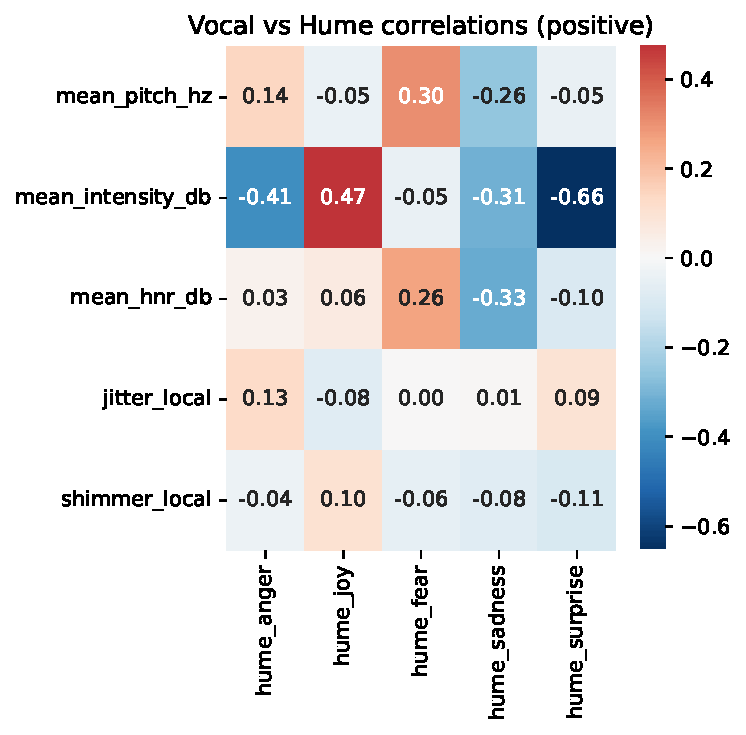
\includegraphics[width=\textwidth]{png/results/rq1_new/vocal_vs_hume_correlations_positive.pdf}
        \caption{Hume vs vocal features positive}
        \label{fig:hume_vocal_positive}
    \end{subfigure}
    \begin{subfigure}[b]{0.45\textwidth}
        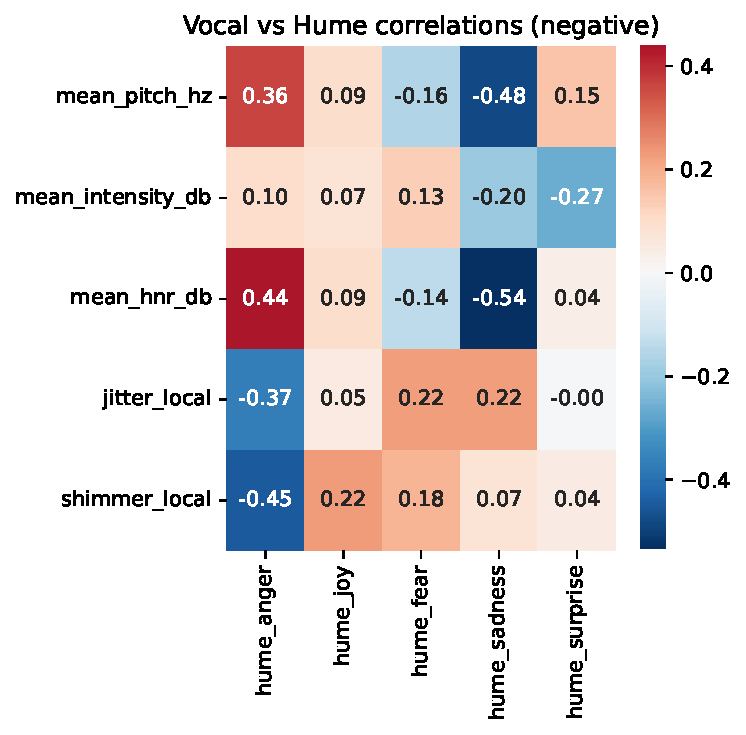
\includegraphics[width=\textwidth]{png/results/rq1_new/vocal_vs_hume_correlations_negative.pdf}
        \caption{Hume vs vocal features negative}        
        \label{fig:hume_vocal_negative}
    \end{subfigure}   
    \caption{Correlation Heatmaps between Hume AI and vocal features.}
    \label{fig:rq1-heatmaps}     
\end{figure}
Correlation values for positive interviews in Figure \ref{fig:hume_vocal_positive} ranging roughly between -0.7 and 0.5, most values suggest generally weaker correlations than the highest values. 
Mean intensity stands out from other vocal features with a moderate positive correlation with Hume Joy (r = 0.47), a moderate negative correlation with Hume Anger (r = -0.41), and a strong negative correlation with Hume Surprise (r = -0.66). 
Mean pitch shows strongest effect on Hume Fear (r = 0.30) and a moderate negative link with Hume Sadness (r = -0.26). 
Mean HNR has a moderate negative correlation with Hume Sadness (r = -0.33) as well it is moderately positively correlated with Hume Fear (r = 0.26). 
Jitter and shimmer remain near zero for most emotions in the positive clips, with none exceeding |r| = 0.13. This suggests that, in more positively oriented interviews, 
variation in pitch, intensity, and HNR capture the core emotion-related cues moderately, while jitter and shimmer have small predictive influence in semi-spontaneous speech during interview conversations. 

Figure \ref{fig:hume_vocal_negative} illustrates Pearson correlation values for negative clips in the dataset, again presenting generally weak effects even if slightly stronger correlations occur, ranging between -0.6 to 0.5. 
The strongest relationship appears for sadness, where mean HNR shows a strong negative correlation (r = -0.54) and pitch has a moderate negative correlation (r = -0.48). The most even distribution of correlation values appear for Hume Anger, 
where all features except intensity shows moderate correlations, most distinct are a positive link with HNR (r = 0.44) and a negative link for shimmer (r = -0.45). Intensity shows overall weak correlations with all emotions, exclusive of Hume Surprise where a moderate negative correlation (r = -0.27) occurs. 
Jitter and shimmer show similar relationships to Hume Fear (r ≈ 0.2). Shimmer has strongest correlation with Hume Anger, and a moderate relationship with Hume Joy. Jitter is moderately correlated with Anger as well and have a moderate correlation with Sadness where shimmer has almost no correlation. 
Pitch and HNR shows the strongest indicators for signalling negative expressed emotions, while intensity measures remain subtle. The slightly strong, but moderate negative correlation between pitch and sadness indicates that the sadder the recording is judged by Hume AI, the lower the average pitch tends to be. 
Both Joy and Surprise has generally weak correlations for all vocal features in the negative oriented clips, which is expected due to these emotions being more positively related. 

\medskip
Overall, the negative and positive diversion suggests that pitch and harmonicity (HNR) consistently reflect Hume AI’s sadness and anger ratings, while intensity mostly marks joy and surprise in positive interviews. Jitter and shimmer remain minor indicators for both interview conditions, except for Anger in the negative clips. 

\subsection{Correlation with Praat-Based Emotion Scores}

\begin{figure}[H]
    \centering 
    \begin{subfigure}[b]{0.45\textwidth}
        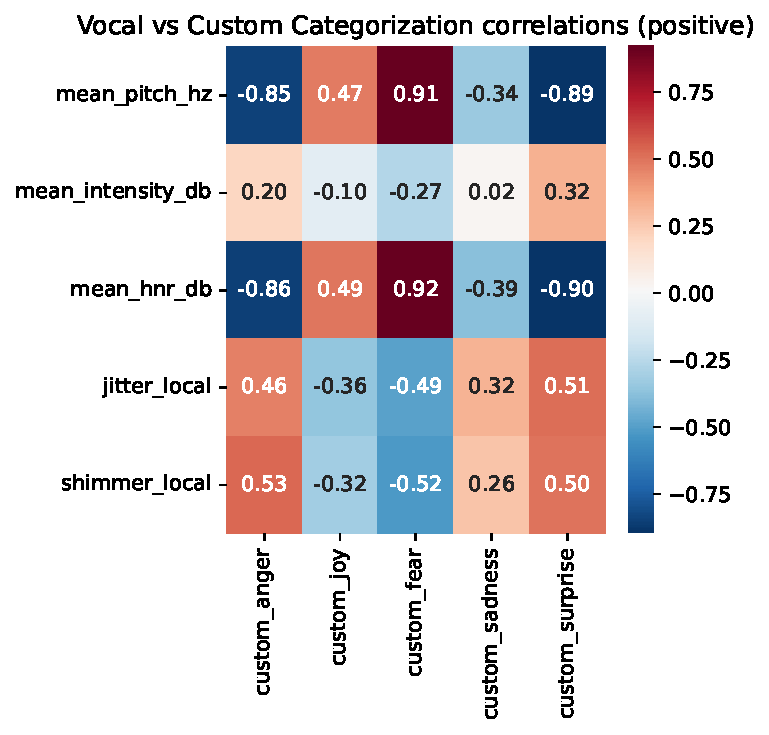
\includegraphics[width=\textwidth]{png/results/rq1_new/vocal_vs_custom_categorization_correlations_positive.pdf}
        \caption{Hume vs custom features positive}
        \label{fig:custom_vocal_positive}
    \end{subfigure}
    \begin{subfigure}[b]{0.45\textwidth}
        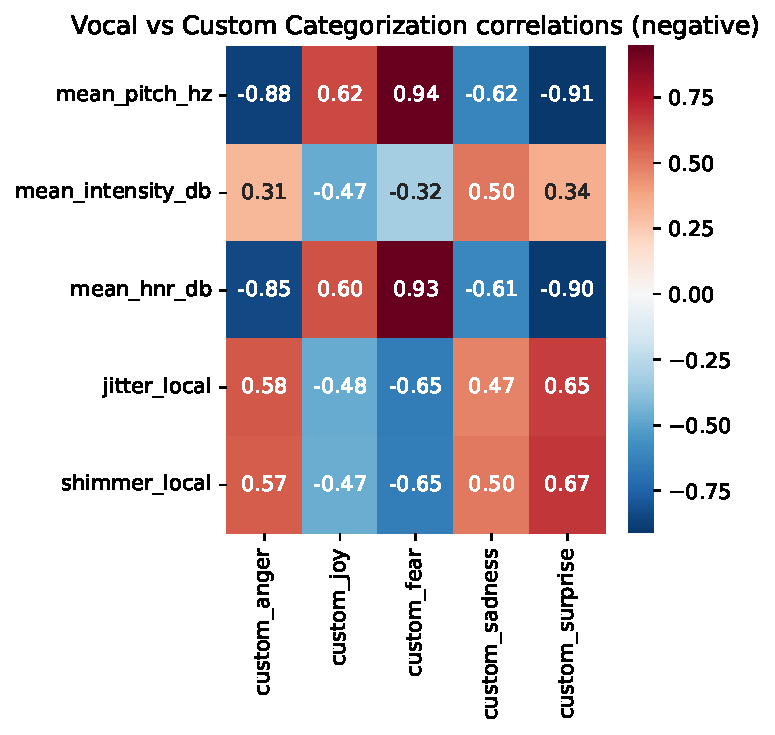
\includegraphics[width=\textwidth]{png/results/rq1_new/vocal_vs_custom_categorization_correlations_negative.pdf}
        \caption{Hume vs custom features negative}        
        \label{fig:custom_vocal_negative}
    \end{subfigure} 
    \caption{Correlation heatmaps between the custom emotion categorization function and vocal features.}
    \label{fig:rq1_heatmaps_custom}       
\end{figure}
Figure~\ref{fig:rq1_heatmaps_custom} presents heatmaps of Pearson’s correlation r between selected vocal features and the emotion scores obtained from the custom emotion categorization 
function for Figure \ref{fig:custom_vocal_positive} positive oriented clips and Figure \ref{fig:custom_vocal_negative} negative clips. Correlations are notably stronger than those observed with the Hume AI labels for both subsets, ranging from -0.9 to 0.95. 
In contrast to the correlation results between Hume AI and vocal markers, these heatmaps presents similar values and orientations for both negative and positive recordings. Pitch and HNR correlations are strongly related for both sentiments, especially between 
pitch and custom categorisations Anger (r = -0.85 and r = -0.88), Fear (r = 0.91 and r = 0.94), and Surprise (r = -0.89 and r = -0.91), the correlation values for HNR is almost identical. Both pitch and HNR shows strong positive correlation for Fear, and strong negative relationship with Anger and Surprise. The almost identical value for these vocal features implies that harmonic clarity is weighted almost identically to pitch in the categorization function, both with a dominant impact on the outcomes of the emotion categorisation. Intensity has a smaller impact, with slightly higher correlations for the negative clips. 
Intensity has weak to moderate relationships across all emotions in the positive recordings, while being strongly correlated with sadness in the negative interviews. The opposite is implied for joy in these interviews, where joy is associated with lower intensity values. 
Jitter and shimmer have slightly stronger correlations across all emotions in the negative oriented clips, yet the values follow the same pattern regarding direction and scale. 

\medskip
These results show that the custom categorization function disproportionately weighted certain vocal features, particularly pitch and HNR, distributing inflating and potentially misleading correlation coefficients. Intensity, shimmer, and jitter has secondary roles with general moderate correlations, although strong correlations appear these features are overwhelmed by pitch and HNR. The almost identical patterns across the sentiment subsets implies overreliance on acoustic features, probably suppressing more subtle cues that are necessary for identifying emotions in semi-spontaneous, conversational speech. 


\subsection{Limitations of the Custom Vocal Emotion Categorization Method}
To evaluate the performance of our custom emotion categorization function, which was developed based on vocal markers reported in the Swedish study \autocite{Ekberg2023}, we compared the emotion labels to the labels generated by Hume AI’s speech-based emotion recognition model. This comparison included both individual clip level and across the full dataset, seperated by sentiment. 

However, the results revealed significant limitations in our approach. Regardless of the vocal input from our dataset, the categorization function consistently rendered near homogeneous emotion scores across all five emotions. This indicates that the function failed to capture emotional distinctions within spontaneous, conversational speech during interviews, regardless of theoretical relevance. 

Figure~\ref{fig:rq1_scatter_hume_praat_pos}, positive, and Figure~\ref{fig:rq1_scatter_hume_praat_neg}, negative, illustrates this issue across the full dataset, where the average scores assigned by our Praat-based categorization remain clustered around 0.2 across all emotions. Opposed to Hume that had greater variation through its labeling and reflects a more dynamic emotional detection.

\begin{figure}[H]
    \centering
    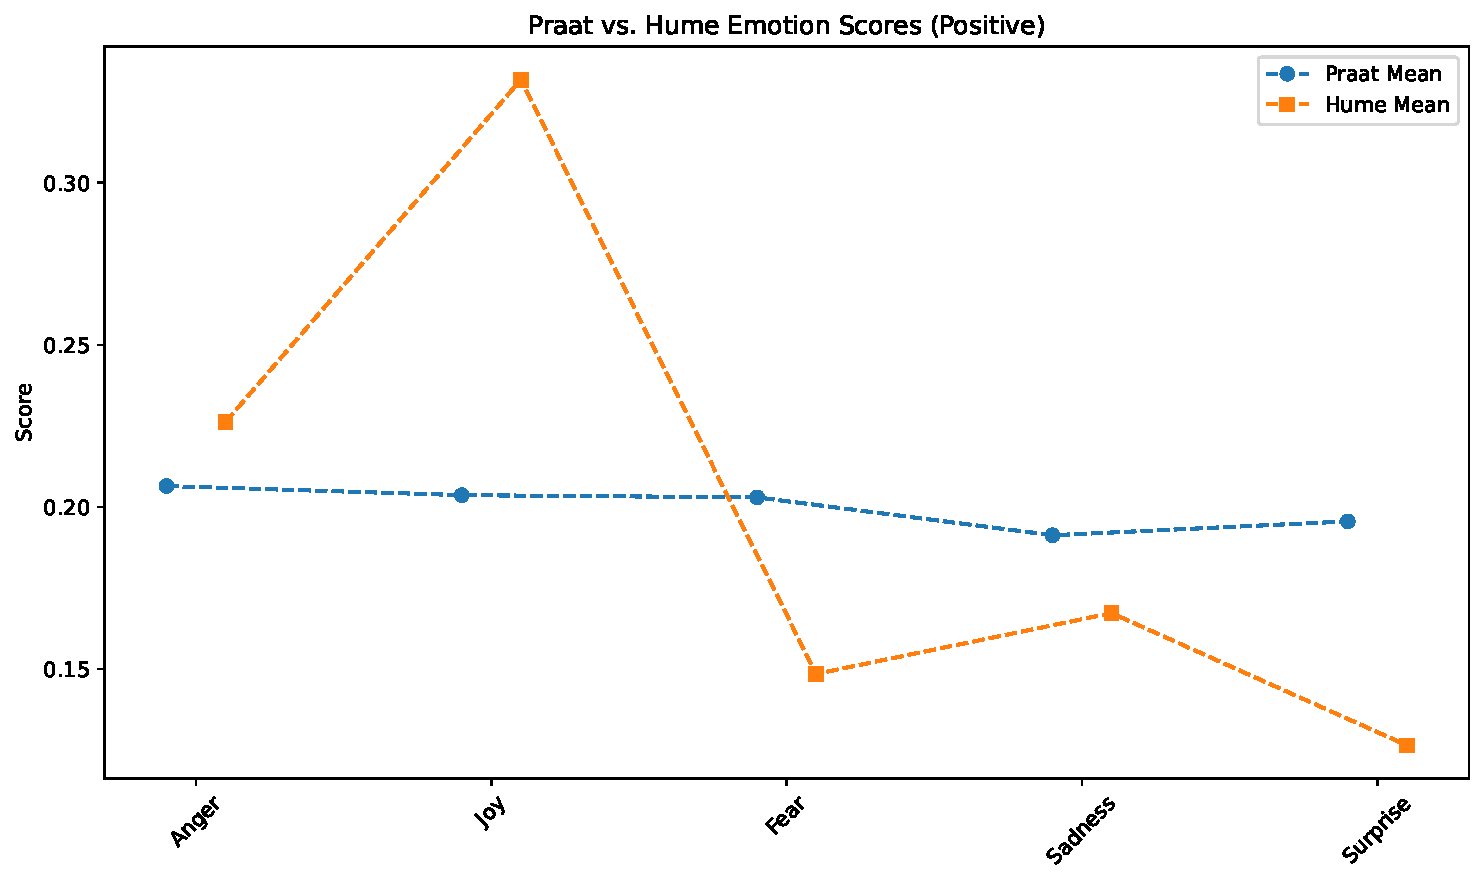
\includegraphics[width=0.75\textwidth]{png/results/rq1_new/praat_hume_positive_scatter.pdf}
    \caption{Average score of custom emotion categorisation function and Hume labeling across positive clips.}
    \label{fig:rq1_scatter_hume_praat_pos}
\end{figure}


\begin{figure}[H]
    \centering
    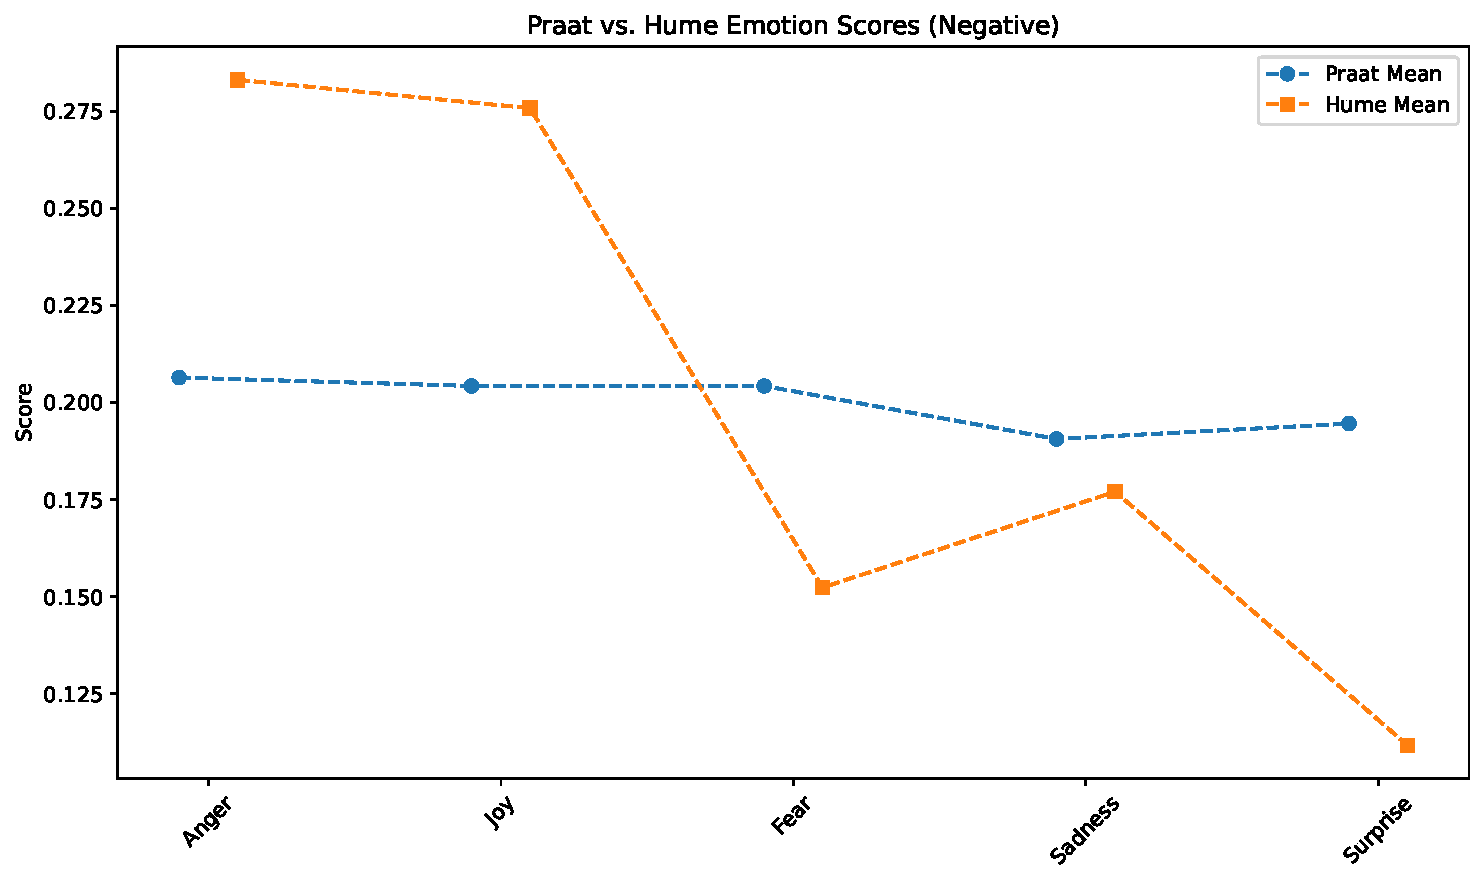
\includegraphics[width=0.75\textwidth]{png/results/rq1_new/praat_hume_negative_scatter.pdf}
    \caption{Average score of custom emotion categorisation function and Hume labeling across negative clips.}
    \label{fig:rq1_scatter_hume_praat_neg}
\end{figure}

    
This is presented similarly in Figure~\ref{fig:praat_hume_006_comb}, which presents a comparison for a single negative 
directed interview \texttt{id\_008\_neg}. In the same way as in Figure~\ref{fig:rq1_scatter_hume_praat_pos} and \ref{fig:rq1_scatter_hume_praat_neg}, 
the Praat-based scores are distributed very evenly across all emotions, while Hume assigns a higher probability to anger and lower for surprise for negative recordings and significantly higher joy scores for positive clips.
Despite the fact that the score diversity between the Hume-labeled emotions are relatively 
moderate, as presented in Figure~\ref{fig:praat_hume_006_comb} comparing one participant's two interviews - approximately 0.05 between anger and fear for the positive clip \ref{fig:praat_hume_006_pos}, yet a differentiation of roughly 0.2 between the highest (fear) and the lowest (surprise) rated emotions. 
The negative interview in Figure~\ref{fig:praat_hume_006_neg} illustrates similar tendencies, with highest probability for anger ($\approx 0.30$) and lowest for surprise (>0.10). 
As both figures in \ref{fig:praat_hume_006_comb} depicts, some alignment occur, yet the probabilities are still more diverse and provide a more interpretable output than yielded from the custom emotion categorisation function. 
The variability could be considered more reflective of potential emotional nuances in the recorded speech. 

These findings demonstrate that our vocal feature-based categorization lacked sensitivity and adaptability when applied to our interview-based Swedish speech data. 
As a result, subsequent analyses focused on direct comparisons between raw vocal features and AI-predicted emotions. 

\begin{figure}[H]
    \centering
    \begin{subfigure}[b]{0.45\textwidth}
        \centering
        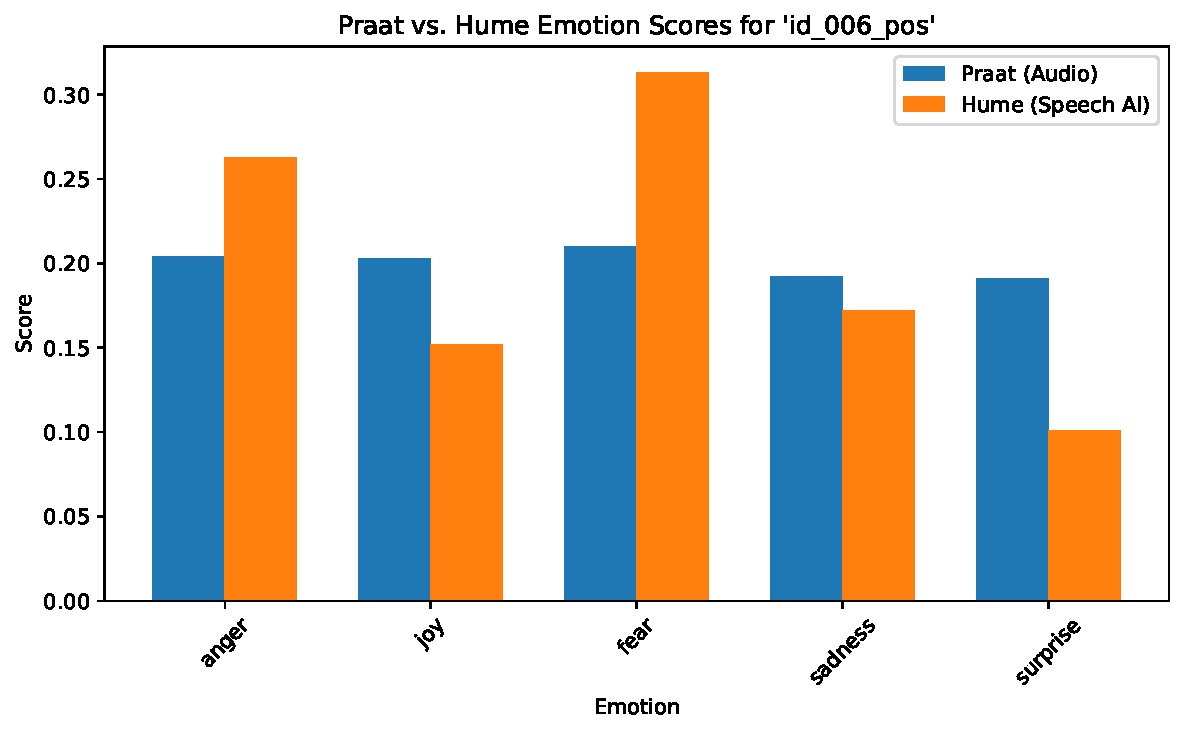
\includegraphics[width=0.7\textwidth]{png/results/rq1_new/id_006_pos_praat_hume_comparison.pdf}
        \caption{Comparison bar single positive clip.}
        \label{fig:praat_hume_006_pos}
    \end{subfigure} 
    \begin{subfigure}[b]{0.45\textwidth}
        \centering
        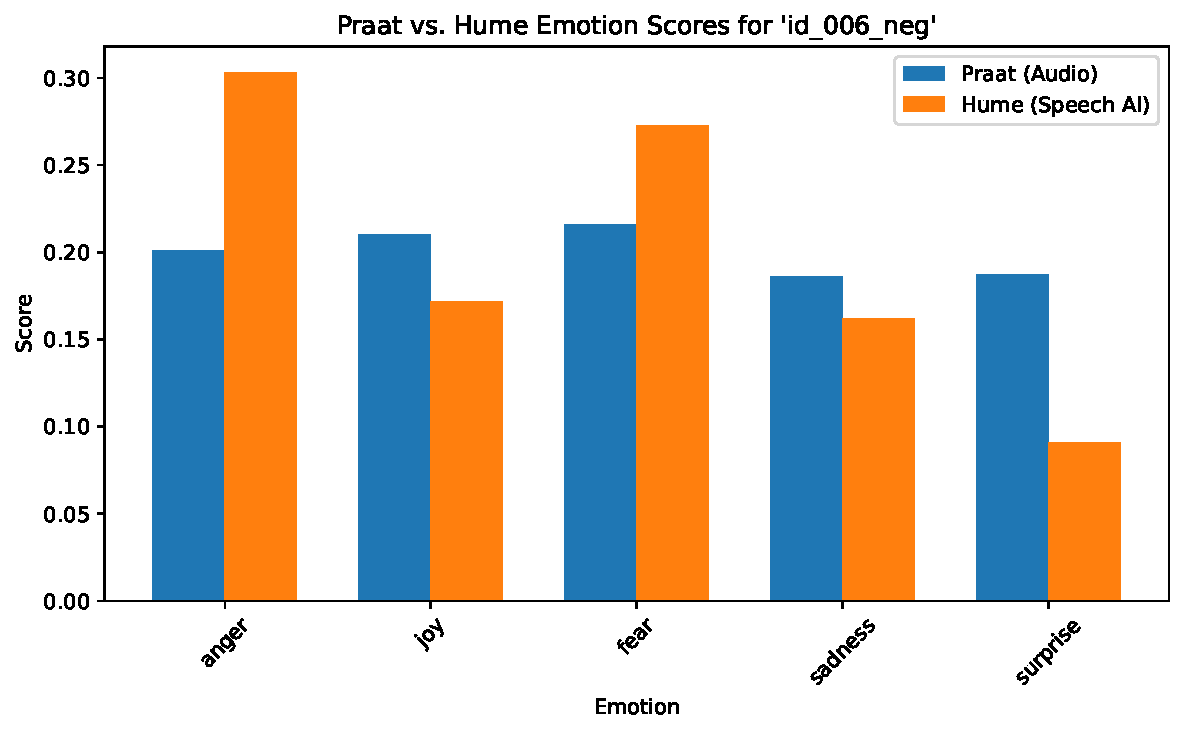
\includegraphics[width=0.7\textwidth]{png/results/rq1_new/id_006_neg_praat_hume_comparison.pdf}
        \caption{Comparison bar single negative clip.}
        \label{fig:praat_hume_006_neg}
    \end{subfigure} 
    \caption{Custom emotion categorization vs. Hume for a single clip (id 006).}
    \label{fig:praat_hume_006_comb}
\end{figure}

\subsection{ANOVA Tables of Vocal Features Across Emotions}
An ANOVA was implemented to further examine whether essential vocal features varied across AI-labeled emotions. This was conducted on pitch, intensity, HNR, jitter, and shimmer. 
The results are summarised in Table~\ref{tab:rq1_anova_pos} for positive recordings and \ref{tab:rq1_anova_neg} for negative recordings, 
showing that none of the features showed statistically significant differences between the five Hume emotion categories (all p-values > 0.30). To confirm these findings, Tukey HSD tests were conducted and resulted in no pairwise comparisons between emotion labels with significant difference. 

\begin{table}[H]
    \centering 
    \begin{subtable}[b]{0.48\textwidth}
        \centering
        \caption*{\textbf{Positive recordings}}
        \begin{tabular}{lrr}
        \toprule
        \multicolumn{1}{c}{\textbf{Feature}} & \textbf{P-value} & \textbf{Significant} \\
        \midrule
        Pitch      & 0,726 & No \\
        Intensity  & 0,812 & No \\
        HNR        & 0,607 & No \\
        Jitter     & 0,954 & No \\
        Shimmer    & 0,731 & No \\
        \bottomrule
        \end{tabular}
        \caption{ANOVA: Positive recordings.}
        \label{tab:rq1_anova_pos}
    \end{subtable}
    \hfill
    \begin{subtable}[b]{0.48\textwidth}
        \centering
        \caption*{\textbf{Negative recordings}}
        \begin{tabular}{lrr}
        \toprule
        \multicolumn{1}{c}{\textbf{Feature}} & \textbf{P-value} & \textbf{Significant} \\
        \midrule
        Pitch      & 0,470 & No \\
        Intensity  & 0,640 & No \\
        HNR        & 0,300 & No \\
        Jitter     & 0,780 & No \\
        Shimmer    & 0,567 & No \\
        \bottomrule
        \end{tabular}
        \caption{ANOVA: Negative recordings.}
        \label{tab:rq1_anova_neg}
    \end{subtable}
    \caption{ANOVA for vocal features across emotions.}
    \label{tab:rq1_anova_all}
\end{table}  
  
These results imply that within our dataset of spontaneous speech during interviews, the average values of the acoustic features did not systematically vary according to AI-labeled emotions. 

OBS! Lägg till medelvärde osv i detta för varje feature (medel och standardavvikelse! )

\subsection{Correlation Between Vocal Features and Hume AI Emotion Scores}
Considering the limitations that had been identified in our vocal feature-based emotion categorization function, subsequent analyses shifted focus towards examining direct correlation between raw acoustic features and AI-predicted emotions. Instead of applying predefined vocal emotion mappings to rely on, essential vocal markers have been investigated to obtain an understanding of how these correlate with Hume AI’s emotion scores across our dataset. 

\subsubsection{Composite Correlation Overview}
Figure~\ref{fig:rq1_composite} illustrates a composite correlation analysis, including Pearson correlation coefficients (r) between two acoustic features, pitch and intensity, and the emotion probabilities from Hume AI. 

\begin{figure}[H]
    \centering 
    \begin{subfigure}[b]{0.48\textwidth}
        \centering
    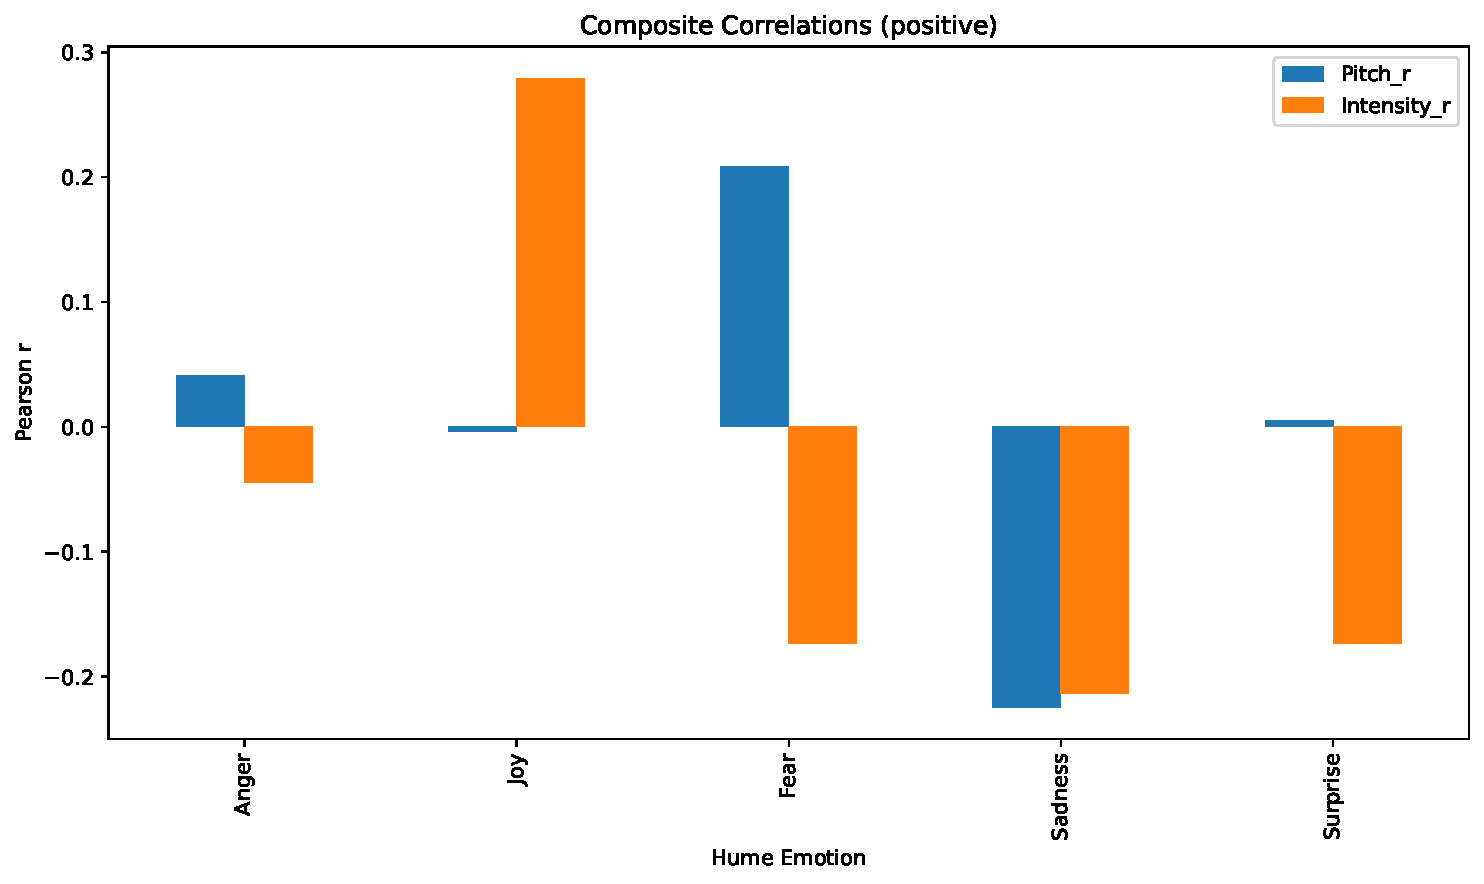
\includegraphics[width=\textwidth]{png/results/rq1_new/composite_correlations_positive.pdf}
    \caption{Positive Recordings}
    \label{fig:rq1_composite_pos}
    \end{subfigure}
    \hfill 
    \begin{subfigure}[b]{0.48\textwidth}
        \centering
        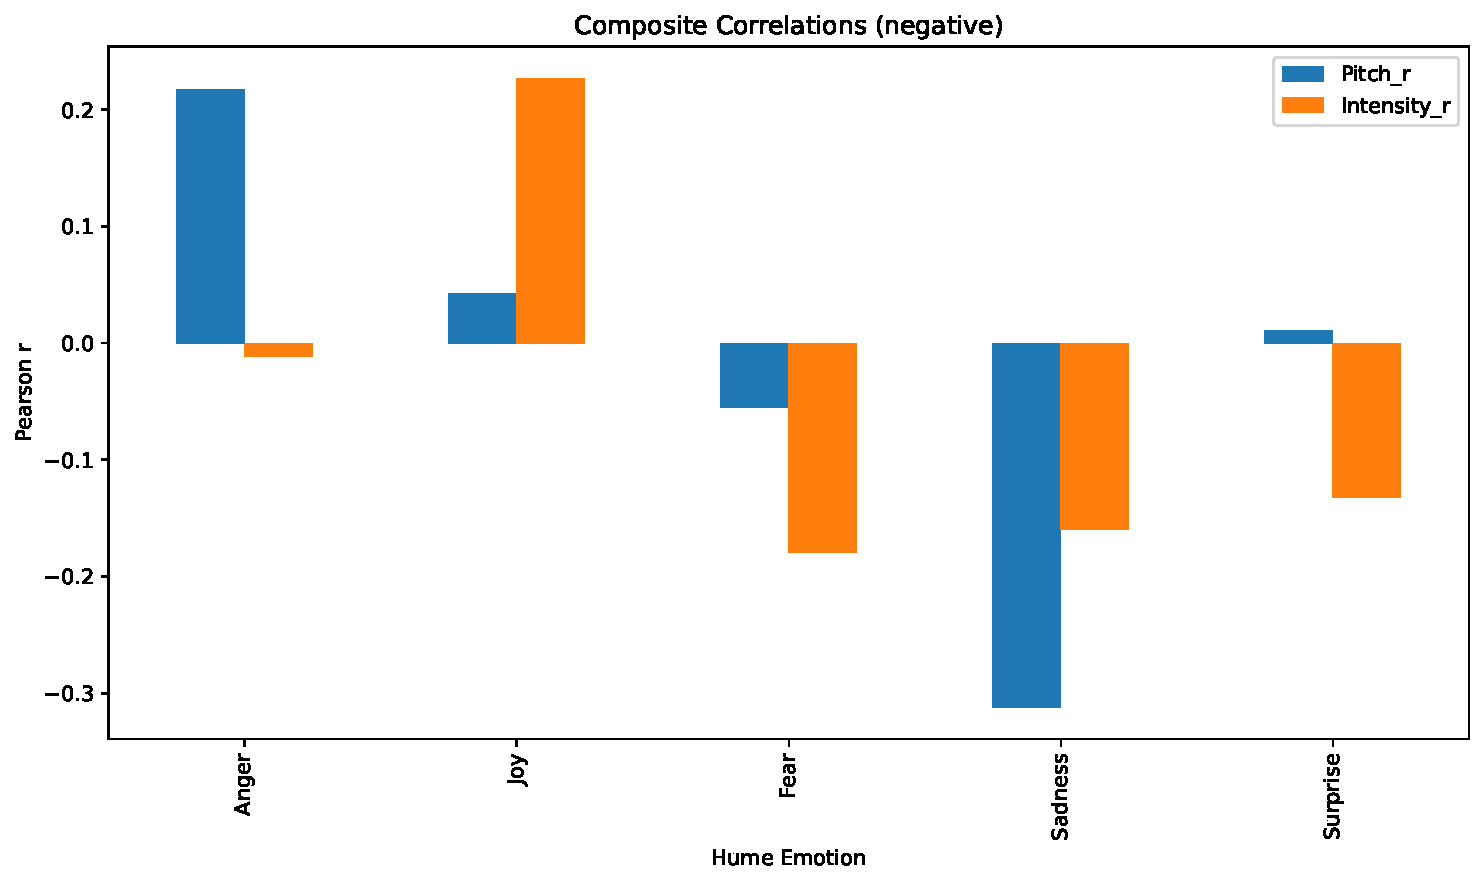
\includegraphics[width=\textwidth]{png/results/rq1_new/composite_correlations_negative.pdf}
    \caption{Negative Recordings}
    \label{fig:rq1_composite_neg}
    \end{subfigure}
    \caption{Composite Correlation diagrams.}
    \label{fig:rq1_composite}
\end{figure}

\begin{table}[H]
    \centering
    \begin{tabular}{lrrrr}
      \toprule
      \textbf{Hume Emotion} & \textbf{Pitch\_r} & \textbf{Pitch\_p} & \textbf{Intensity\_r} & \textbf{Intensity\_p} \\
      \midrule
      Anger    & 0,218 & 0,000 & –0,012 & 0,762 \\
      Joy      & 0,042 & 0,282 &  0,227 & 0,000 \\
      Fear     & –0,055 & 0,159 & –0,180 & 0,000 \\
      Sadness  & –0,312 & 0,000 & –0,160 & 0,000 \\
      Surprise & 0,011 & 0,788 & –0,132 & 0,001 \\
      \bottomrule
    \end{tabular}
    \caption{Correlation coefficients (r) and p-values for pitch and intensity, negative recordings. }
    \label{tab:cor_neg}
  \end{table}
  
Pitch in negative recordings shows a positive correlation with Hume anger (r = 0.218, p < 0.001) and a negative correlation with Hume sadness (r = -0.312, p < 0.001), both showing statistical significance. 
Other emotions presents no significant correlation, where pitch and surprise has the weakest correlation across emotions. Intensity correlates positively with Hume joy (r = 0.227) and had a negative relationship with fear (r = -0.180), sadness (r = -1.60), and surprise (r = -0.132), all statistical significant correlations (p < 0.01). 
Anger was the single emotion showing weak correlation with intensity (r = -0.012, p = 0.762) across the negative interviews. 

  \begin{table}[H]
    \centering
    \begin{tabular}{lrrrr}
      \toprule
      \textbf{Hume Emotion} & \textbf{Pitch\_r} & \textbf{Pitch\_p} & \textbf{Intensity\_r} & \textbf{Intensity\_p} \\
      \midrule
      Anger    & 0,041 & 0,362 & –0,045 & 0,320 \\
      Joy      & –0,004 & 0,936 &  0,279 & 0,000 \\
      Fear     & 0,209 & 0,000 & –0,173 & 0,000 \\
      Sadness  & –0,225 & 0,000 & –0,213 & 0,000 \\
      Surprise & 0,005 & 0,916 & –0,173 & 0,000 \\
      \bottomrule
    \end{tabular}
    \caption{Correlation coefficients (r) and p-values for pitch and intensity, positive recordings. }
    \label{tab:cor_pos}
  \end{table}

Both fear and sadness predicted by Hume AI showed weak correlations with statistical significance with pitch for positive recordings (r = 0.209 and r = -0.225, both p < 0.001). All other pitch correlations were non-significant. 
Intensity correlated most strongly with joy (r = 0.279, p < 0.001), and strongest negatively with sadness (r = -0.213, p < 0.001). Weak correlations with statistical significance were also prevelant between intensity and fear (r = -0.173, p < 0.001) and surprise (r = -0.173, p < 0.001).


\subsubsection{OBS!!! DELETE!!! should be in discussion!!!! }


Particularly intensity shows a positive correlation with joy, and suggests that higher vocal intensity tends to co-occur with AI detected happiness. In contrast, intensity shows a negative correlation with emotions such as sadness and fear, which is aligned with the expectations that these emotions are generally expressed with lower vocal energy. 

For pitch, a minor positive correlation is found in correlation with anger and fear, also reflecting expectations reported in prior research, where higher pitch is associated with heightened arousal states, for example anger. A negative correlation between pitch and sadness is shown, also supporting the prior findings where sadness is linked to lower pitch. 

However, the correlation strength is weak across all emotions, without values that indicate a strong linear association. This indicates, as our previous results, that single acoustic features like pitch and intensity alone are insufficient markers of emotional states when detected by speech emotion recognition systems, in the context of conversational, but interviewed, speech. 

\subsection{Time-to-Time Analysis}

For a more concrete illustration of the prior tendencies , two interview recordings were analyzed in detail. The purpose was to examine whether emotional shifts become more apparent when evaluating shorter time segments within individual speakers, compared to the weaker correlations observed at the dataset level.

\medskip

\begin{figure}[H]
    \centering
    
    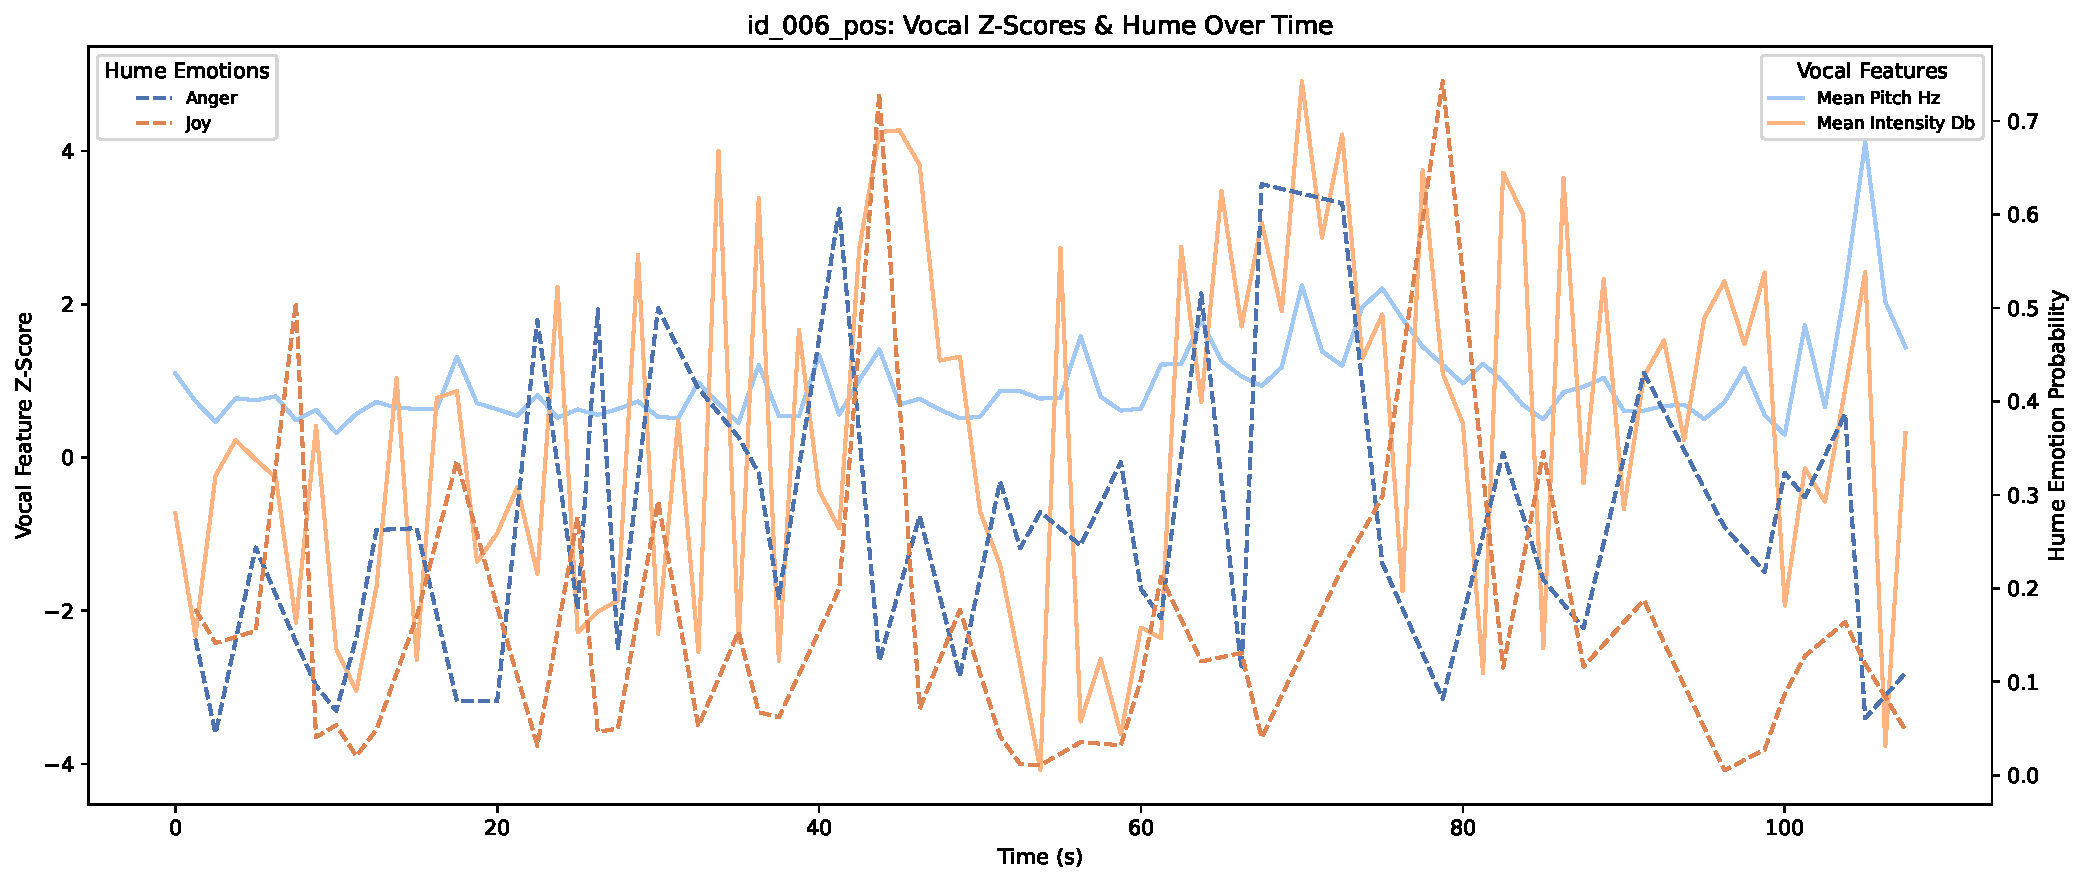
\includegraphics[width=0.85\textwidth]{png/results/rq1_new/006_pos_use_anger-joy.pdf}
    \caption{Pitch and Intensity vs. Hume Anger and Joy. Single positive clip.}
    \label{fig:006_pos-anger-joy}
\end{figure}

\begin{figure}[H]
    \centering
    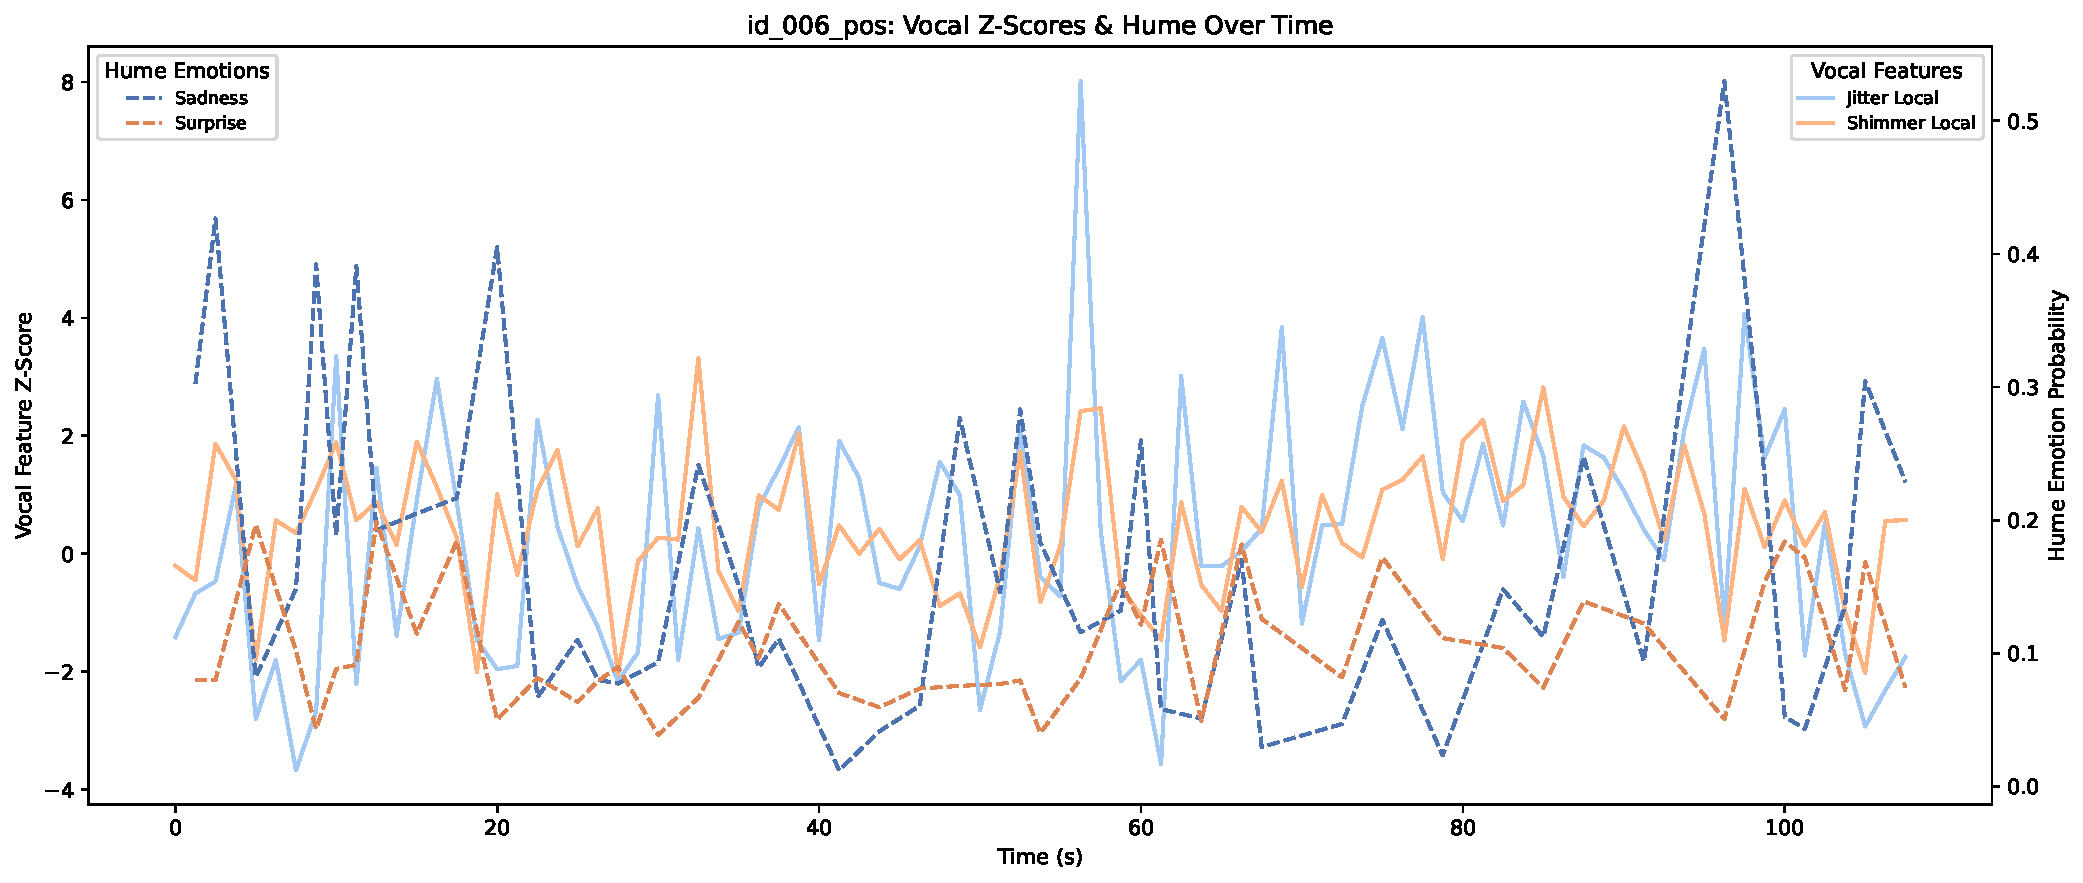
\includegraphics[width=0.85\textwidth]{png/results/rq1_new/006_pos_use-sadn-surp.pdf} 
    \caption{Jitter and Shimmer vs. Hume Sadness and Surprise. Single positive clip.}
    \label{fig:006_pos-surp-sadn}
\end{figure}
    
\begin{table}[H]
    \centering
    %\caption*{\textbf{Significant Correlations}}
    \begin{tabular}{llrr}
        \toprule
        \textbf{Feature}         & \textbf{Emotion} & \textbf{Pearson r} & \textbf{p-value} \\
        \midrule
        mean\_pitch\_st          & surprise         & 0.257              & 0.016            \\
        mean\_pitch\_hz          & surprise         & 0.258              & 0.016            \\
        mean\_intensity\_db      & joy              & 0.271              & 0.011            \\
        mean\_intensity\_db      & fear             & $-0.338$           & 0.001            \\
        \bottomrule
    \end{tabular}
    \caption{Segment-wise Significant Correlations clip 006pos}
    \label{tab:segcorr_significant}
\end{table}

For \ref{tab:segcorr_significant} number of unsignificant: 25 



\begin{table}[H]
    \centering
   % \caption*{\textbf{High vs Low T-tests Statistics}}
    \begin{tabular}{llrr}
        \toprule
        \textbf{Feature}         & \textbf{Emotion} & \textbf{t-statistic} & \textbf{p-value} \\
        \midrule
        mean\_pitch\_st          & surprise         & 2.373                & 0.020            \\
        mean\_pitch\_hz          & surprise         & 2.412                & 0.018            \\
        mean\_intensity\_db      & joy              & 2.399                & 0.019            \\
        \bottomrule
    \end{tabular}
    \caption{High vs Low T-test Statistics (Significant Results) clip 006pos}
    \label{tab:seghighlow_ttest}
\end{table}
  
for \ref{tab:seghighlow_ttest} number unsignificant: 26 

\begin{table}[H]
    \centering
    %caption*{\textbf{Segment wise Slopes for vocal features}}
    \begin{tabular}{lrrl}
        \toprule
        \textbf{Feature}         & \textbf{Slope}  & \textbf{p-value} & \textbf{Significant?} \\
        \midrule
        mean\_pitch\_st          & 0.005           & 0.000            & Yes                  \\
        mean\_pitch\_hz          & 0.007           & 0.000            & Yes                  \\
        mean\_intensity\_db      & 0.019           & 0.016            & Yes                  \\
        mean\_hnr\_db            & 0.003           & 0.061            & No                   \\
        jitter\_local            & 0.015           & 0.033            & Yes                  \\
        shimmer\_local           & 0.002           & 0.632            & No                   \\
        \bottomrule
    \end{tabular}
    \caption{Segment-wise Slopes for Vocal Features clip 006pos}
    \label{tab:segslope_significant}
\end{table}



\begin{figure}[H]
    \centering 
    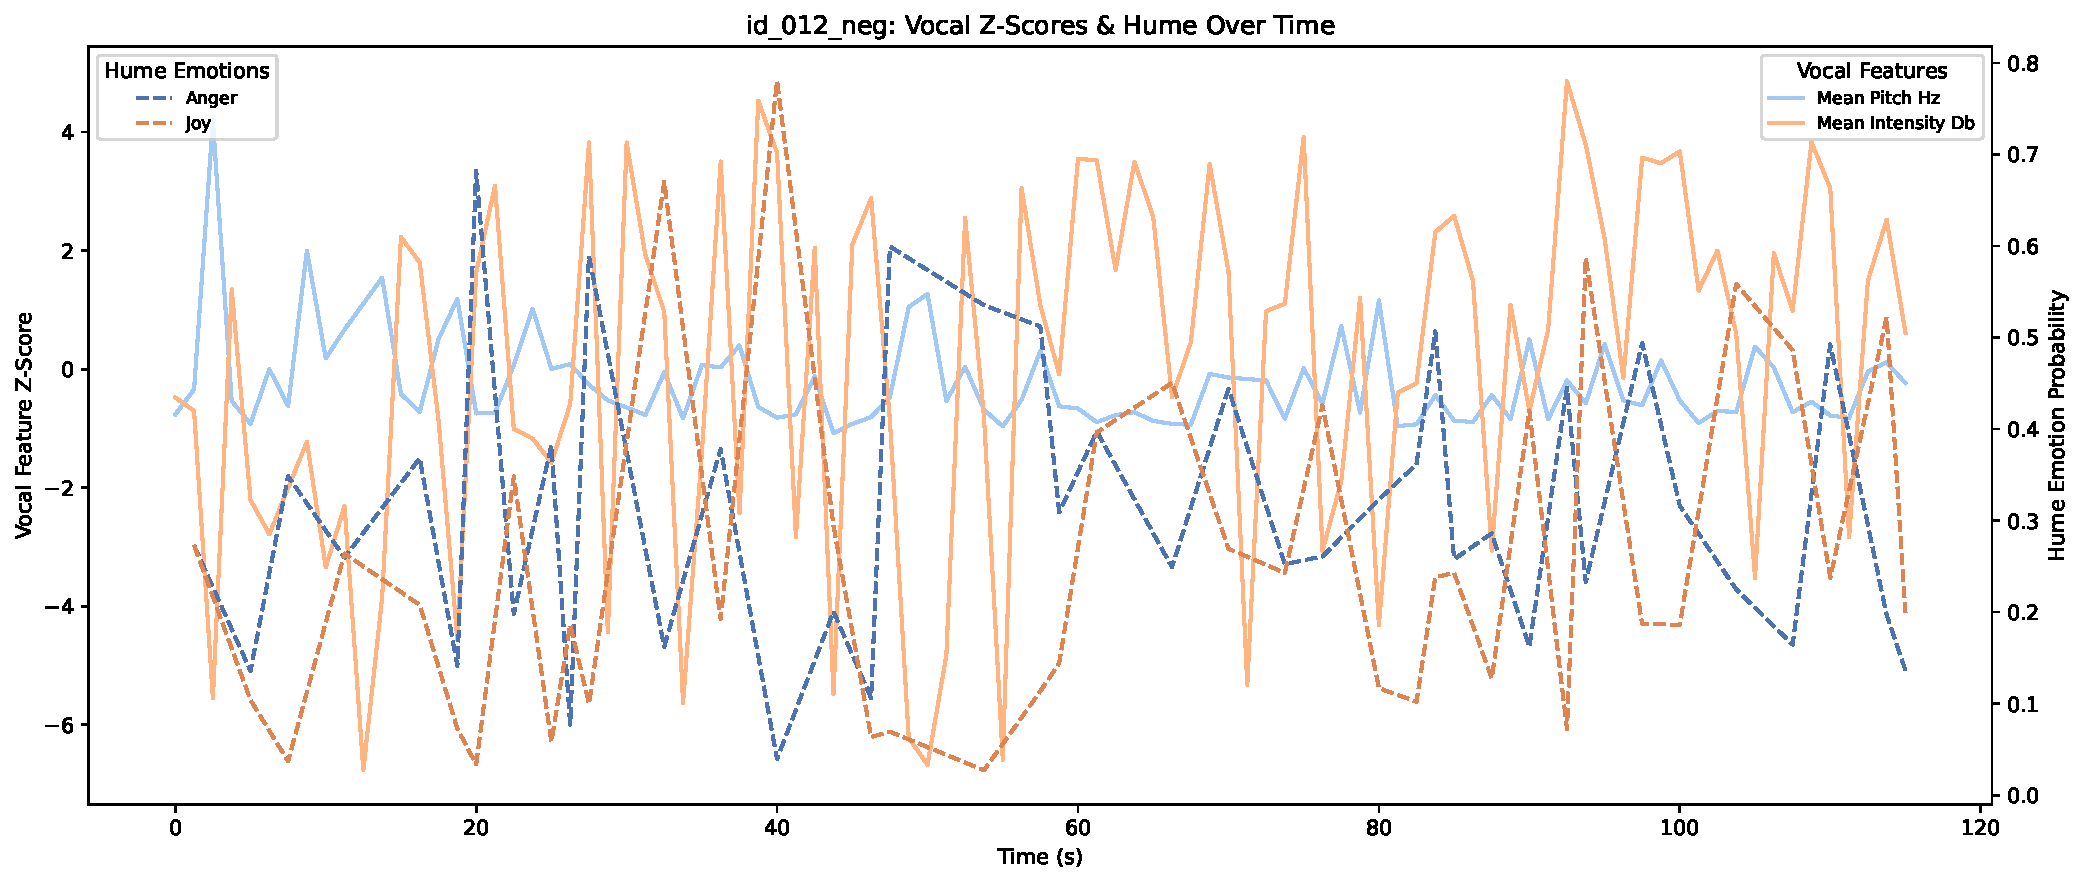
\includegraphics[width=0.85\textwidth]{png/results/rq1_new/012_neg_use-anger-joy.pdf}
    \caption{Z score fluctuation pitch, intensity, anger and joy single clip.}
    \label{fig:z-score-ang-joy-012}
\end{figure}

\begin{figure}[H]
    \centering 
    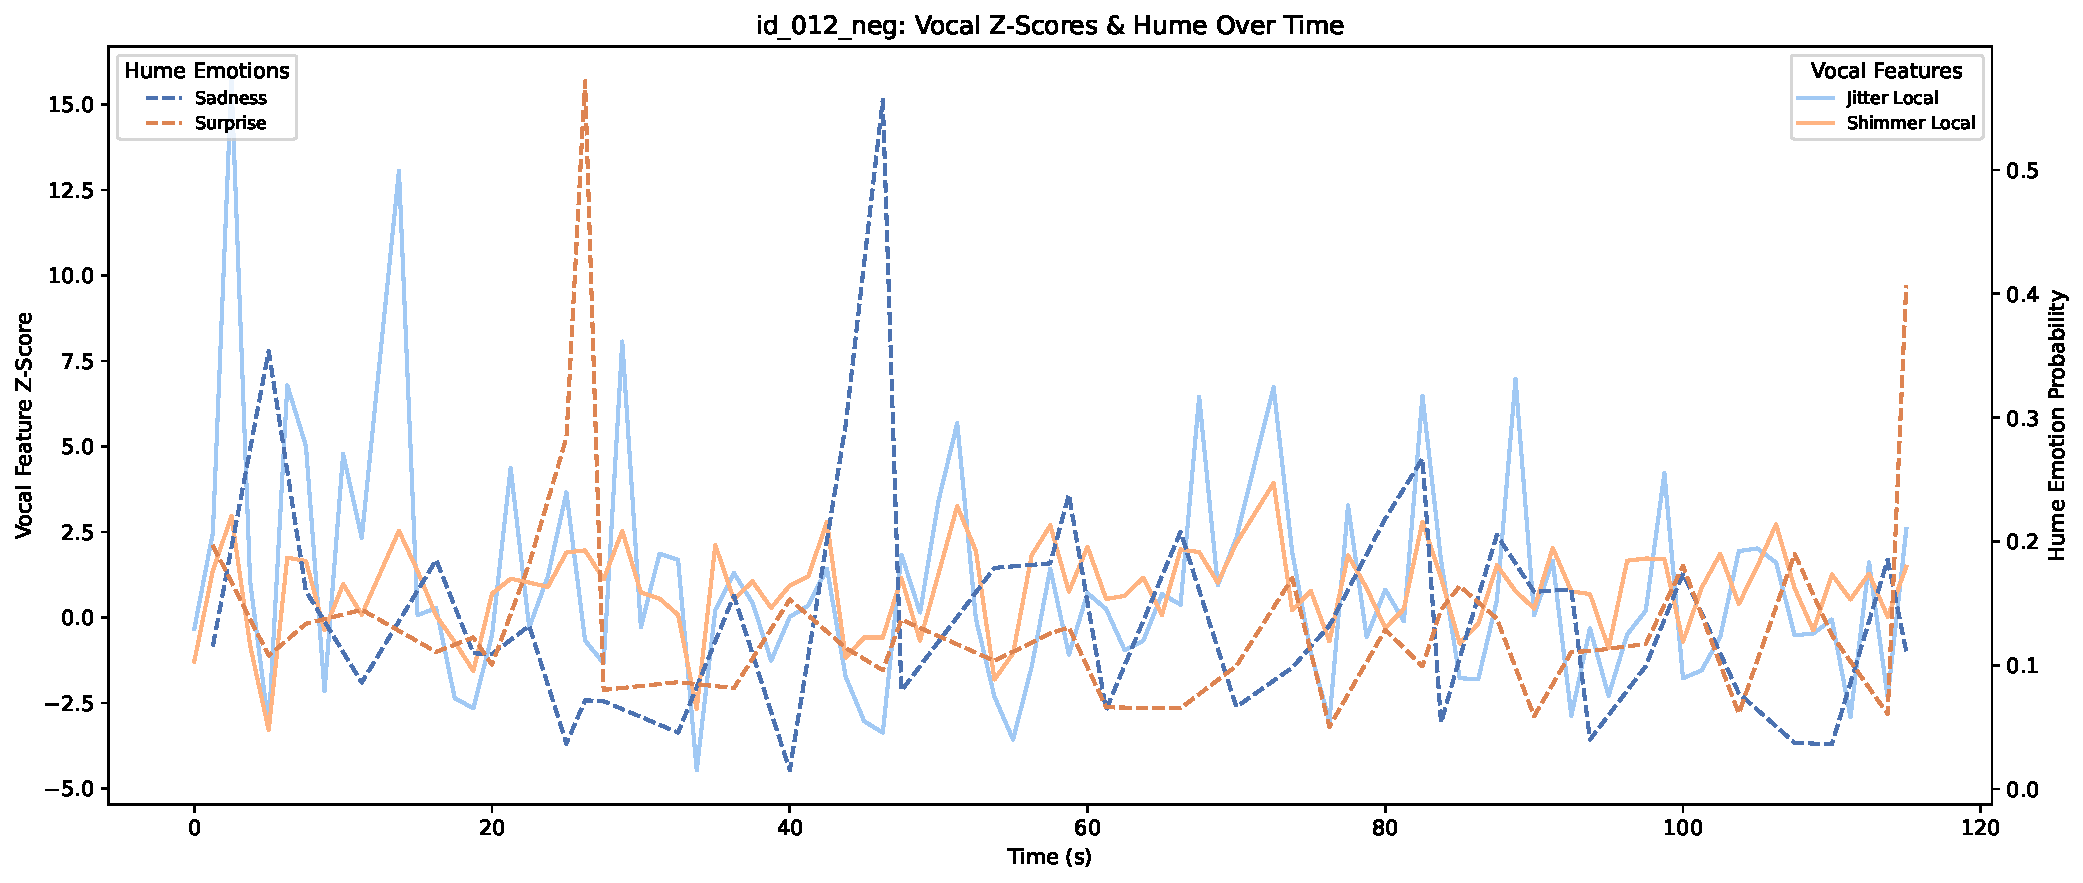
\includegraphics[width=0.85\textwidth]{png/results/rq1_new/012_neg_use-sadn-surp.pdf}
    \caption{Z score fluct jitter, shimmer, sadness, surprise single clip.}
    \label{fig:z-score-surp-sadn-012}
\end{figure}


  \begin{table}[H]
    \centering 
    %\caption*{\textbf{Segment wise correlations : unsig: 25}}
    \begin{tabular}{llrr}
      \toprule
      \textbf{Feature}         & \textbf{Emotion} & \textbf{Pearson r} & \textbf{p-value} \\
      \midrule
      mean\_pitch\_st          & fear             & 0.285              & 0.0063           \\
      mean\_pitch\_hz          & fear             & 0.269              & 0.0099           \\
      mean\_intensity\_db      & fear             & $-0.300$           & 0.0035           \\
      mean\_hnr\_db            & fear             & 0.296              & 0.0040           \\
      mean\_hnr\_db            & surprise         & 0.212              & 0.0417           \\
      \bottomrule
    \end{tabular}
    \caption{Segment-wise Significant Correlations (Fear and Surprise) unsign: 25. clip 012neg}
    \label{tab:segcorr_fear_012}
  \end{table}
  
 
  \begin{table}[H]
    \centering
    \caption*{\textbf{High vs Low T-tests Statistics unsign: 25}}
    \begin{tabular}{llrrr}
      \toprule
      \textbf{Feature}         & \textbf{Emotion} & \textbf{Group}     & \textbf{t-statistic} & \textbf{p-value} \\
      \midrule
      mean\_pitch\_st          & sadness          & High vs Low        & $-2.580$             & 0.0115           \\
      mean\_pitch\_hz          & sadness          & High vs Low        & $-2.343$             & 0.0214           \\
      mean\_hnr\_db            & sadness          & High vs Low        & $-2.397$             & 0.0186           \\
      jitter\_local            & surprise         & High vs Low        & 2.494                & 0.0145           \\
      \bottomrule
    \end{tabular}
    \caption{High vs Low T-test Statistics (Significant Results) unsign: 25 clip 012neg}
    \label{tab:seghighlow_sad_surp_012}
  \end{table}
  

  \begin{table}[H]
    \centering
    \caption*{\textbf{Slope}}
 
    \begin{tabular}{lrrl}
      \toprule
      \textbf{Feature}         & \textbf{Slope}  & \textbf{p-value} & \textbf{Significant?} \\
      \midrule
      mean\_pitch\_st          & $-0.005$        & 0.0207           & Yes                   \\
      mean\_pitch\_hz          & $-0.006$        & 0.0118           & Yes                   \\
      mean\_intensity\_db      & 0.029           & 0.0018           & Yes                   \\
      mean\_hnr\_db            & $-0.005$        & 0.0012           & Yes                   \\
      jitter\_local            & $-0.019$        & 0.0636           & No                    \\
      shimmer\_local           & 0.005           & 0.2496           & No                    \\
      \bottomrule
    \end{tabular}
    \caption{Segment-wise Slopes for Vocal Features clip 012neg}
    \label{tab:segslope_012}
  \end{table}



\subsubsection{Pitch and Hume emotion over time}
In Figure~\ref{fig:pitch-4-pos} and \ref{fig:intensity-4-pos}, data is demonstrated from a positively directed interview \texttt{id\_004\_pos}, female, which shows that increases in pitch and intensity considerably often correlate with higher joy probabilities by Hume AI. While the correlation is not consistent throughout the recording, these moment-to-moment variations reflect the general expectation that higher vocal energy is associated with positive emotional expression. 

\begin{figure}[H]
    \centering
    \begin{subfigure}[b]{0.47\textwidth}
        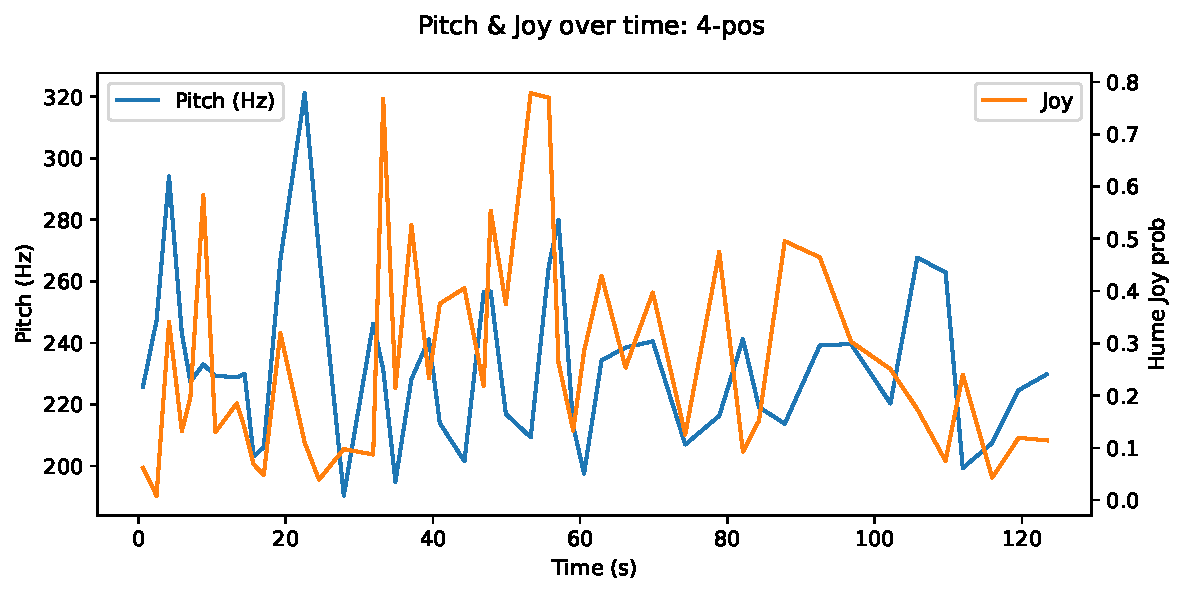
\includegraphics[width=\linewidth]{png/results/rq1/pitch_joy_4-pos.pdf}
        \caption{Pitch(Hz) and Hume label joy over time. Clip 4-pos}
        \label{fig:pitch-4-pos}
    \end{subfigure}
    \hspace{0.04\textwidth}
    \begin{subfigure}[b]{0.47\textwidth}
        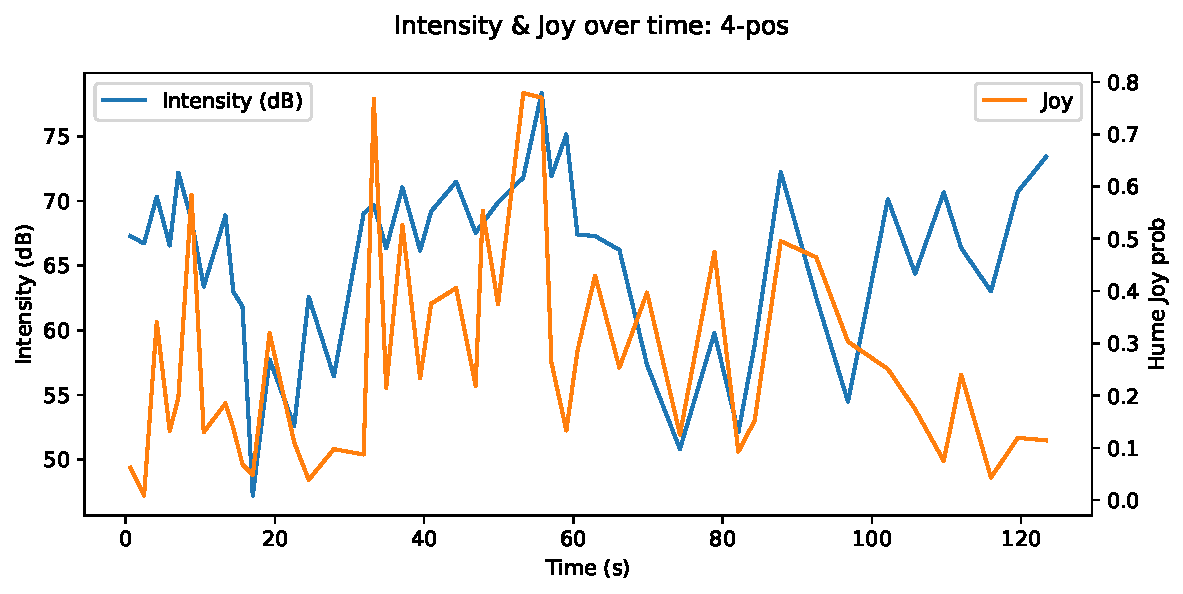
\includegraphics[width=\linewidth]{png/results/rq1/intensity_joy_4-pos.pdf}
        \caption{Intensity(dB) and Hume label joy over time. Clip 4-pos}
        \label{fig:intensity-4-pos}
    \end{subfigure}
\end{figure}

Similarly, Figure~\ref{fig:pitch-15-neg} and \ref{fig:intensity-15-neg} and \ref{fig:z-score-15} present data from a negatively directed interview \texttt{id\_015\_neg}, male. Here, clear peaks in pitch and intensity correspond with increased anger probabilities. These results are partly aligned with prior research on vocal markers of high-arousal negative emotions, such as raised pitch and loudness during expressed anger. 

\begin{figure}[H]
    \centering
    \begin{subfigure}[b]{0.47\textwidth}
        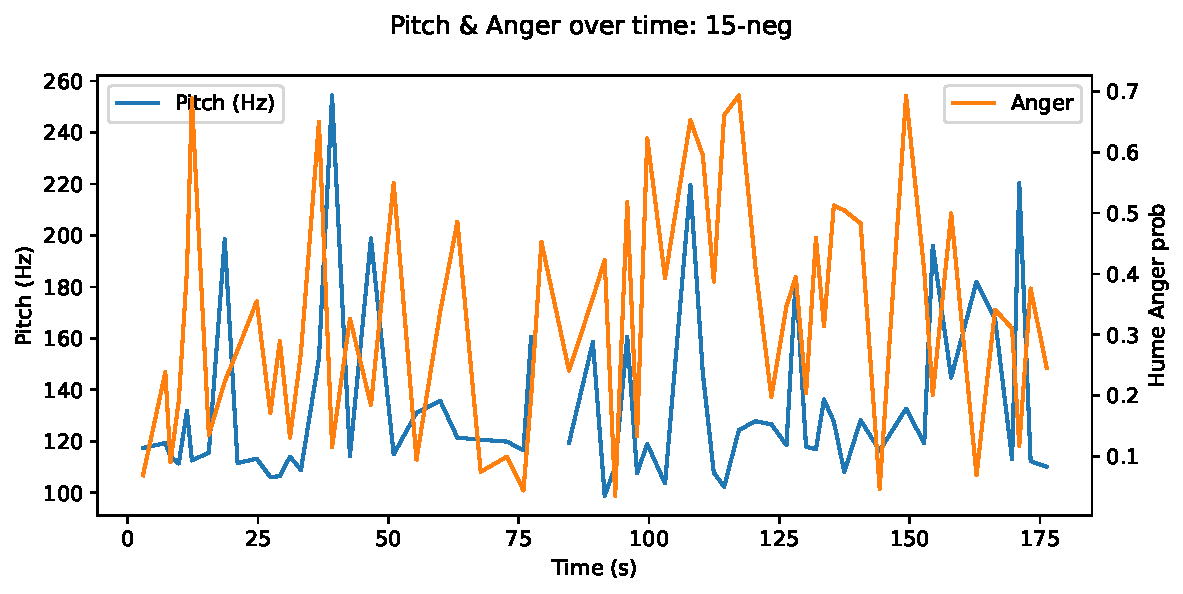
\includegraphics[width=\linewidth]{png/results/rq1/pitch_anger_15-neg.pdf}
        \caption{Pitch(Hz) and Hume label joy over time. Clip 15-neg}
        \label{fig:pitch-15-neg}
    \end{subfigure}
    \hspace{0.04\textwidth}
    \begin{subfigure}[b]{0.47\textwidth}
        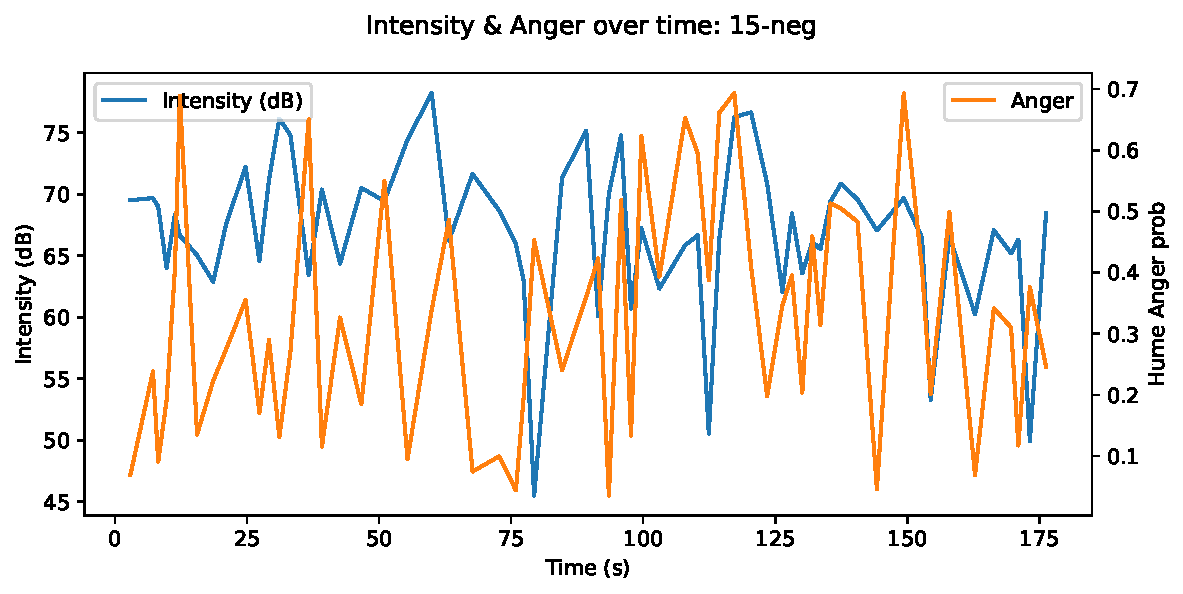
\includegraphics[width=\linewidth]{png/results/rq1/intensity_anger_15-neg.pdf}
        \caption{Intensity(dB) and Hume label joy over time. Clip 15-neg}
        \label{fig:intensity-15-neg}
    \end{subfigure}
\end{figure}

Additionally, Figure \ref{fig:z-score-15} illustrates z-score fluctuations of key vocal features for clip 13-neg. For this interview, several segments exceed +-1 standard deviation from the baseline, especially for pitch, intensity, and shimmer. These flagged moments align frequently with the emotion probabilities of Hume, which strengthens the link between vocal patterns and perceived emotional intensity. 

The z-score fluctuation diagram Figure \ref{fig:z-score-15} illustrates the segments further where vocal features significantly deviate from baseline levels, in patterns aligned with associated high-arousal negative emotions such as raised pitch and loudness. 

\begin{figure}[H]
    \centering 
    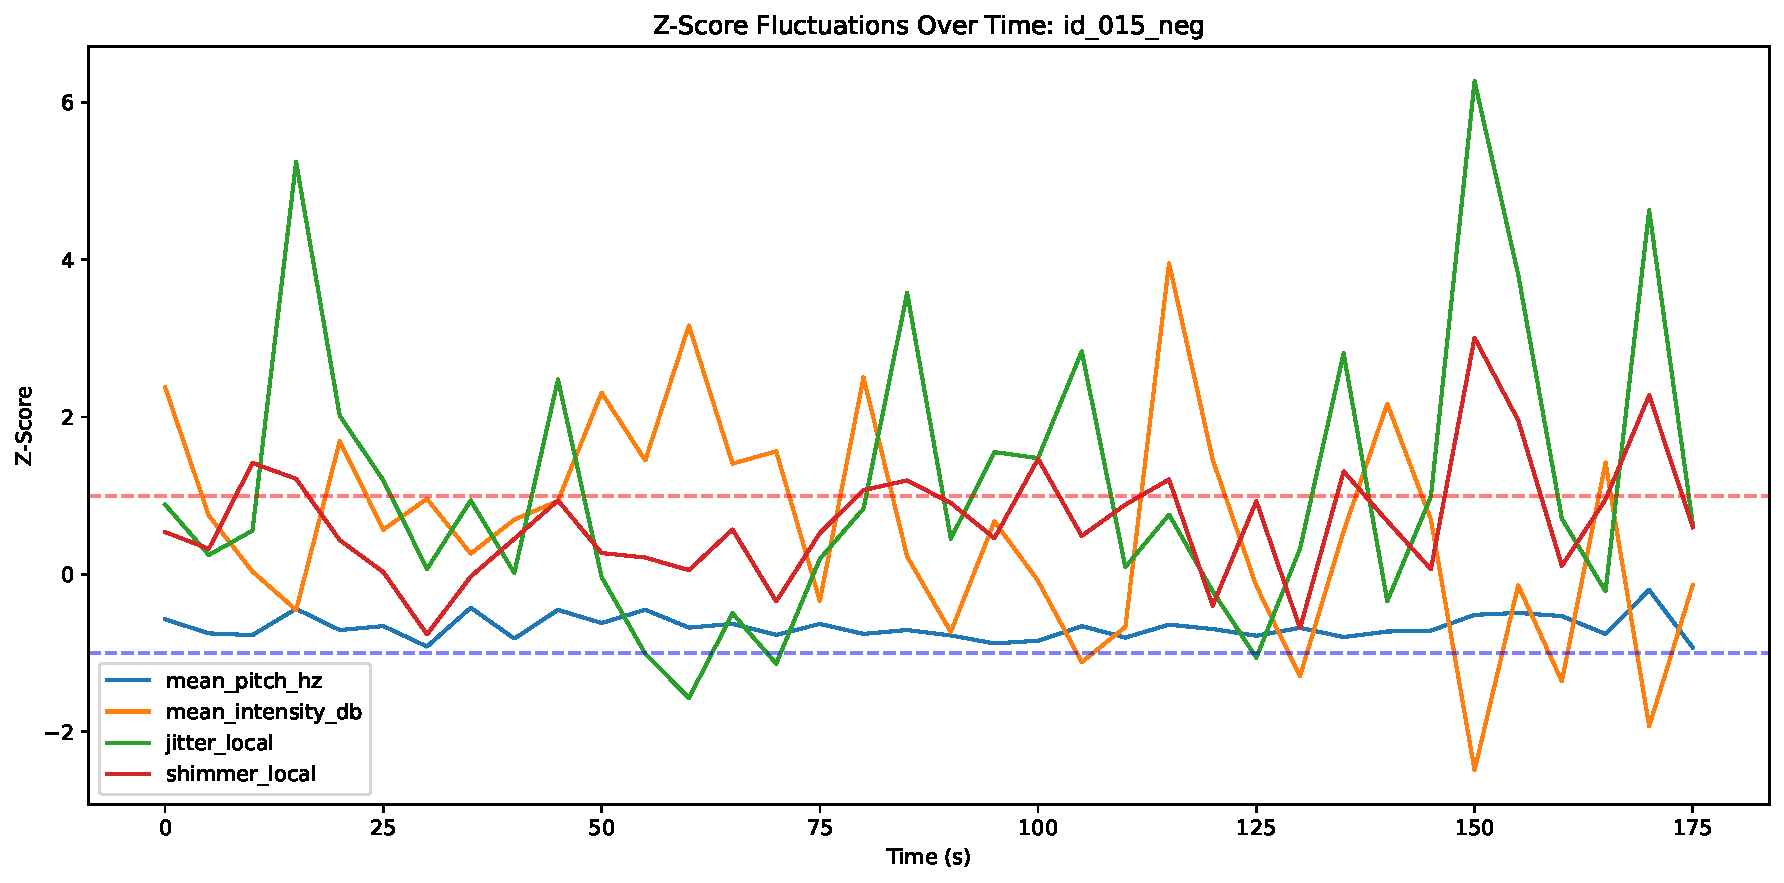
\includegraphics[width=0.7\textwidth]{png/results/rq1/zscore_fluctuations_id_015_neg.pdf}
    \caption{Z-score}
    \label{fig:z-score-15}
\end{figure}

\subsubsection{Summery}
This supports the idea that analyzing how vocal features change over time  can provide more meaningful insights into emotional expression in conversational, partly spontaneous speech during interviews compared to only using overall clip-level statistics.

\subsection{Conclusion RQ1 Data Analysis}
The results revealed only weak to moderate correlations for the analysis between individual vocal features and how Hume AI predicted emotions, where intensity and pitch showed most patterns consistently. 
The custom vocal categorization method did not function well in this context and resulted in very uniform results. This method was built on a basic group of vocal features which may overlooked important indicators for certain emotions. 
ANOVA tests found no significant differences in vocal features across AI-labeled emotions. However, examining pitch and intensity fluctuations over time segments in individual clips gave more promising results. This implies that dynamic changes in vocal features 
can offer more insights than static averages when analysing conversational, yet spontaneous speech during interviews. 

%%%%%%%%%%%%%%%%%%%%%%%%%%%%%%%%%%%%%%%%%%%%%%%%%%%%%%%%%%%%%%%%%%%%%%%%%%%%%%%%%%%%%%%%%%
                        %%%%%%%%%%%% RQ2 %%%%%%%%%%%%%%%%%%
 %%%%%%%%%%%%%%%%%%%%%%%%%%%%%%%%%%%%%%%%%%%%%%%%%%%%%%%%%%%%%%%%%%%%%%%%%%%%%%%%%%%%%%%%%%
\section{Data Analysis for RQ2: Text and Speech Based Emotion Recognition}
Research Question 2 explores how two modalities for AI-based emotion recognition systems - speech-based (Hume AI) and text-based (NLP Cloud) - aligns and diverge in their interpretation of emotional expressions for semi-structured interviews. 
The analysis evaluate the agreement between the models for five basic emotions by comparing average scores, measuring statistical correlation and significance, and exploring how the sentiment context (positive vs. negative) may impact detection. 
This multimethod approach support a comprehensive understanding of how the two modilities responds to the same emotional input, to find mutual strenghs and diverse tendencies in how they classifies emotions. 
\subsection{Overall Comparison of AI Systems}
To compare the overall performance and certain tendencies of the two AI-based emotion recognition systems (Hume AI and NLP Cloud),
both descriptive statistics and visual analyses were conducted to interpret the results through calculating the average differences.

As presented in Table~\ref{tab:summery_rq2_rq3}, Table~\ref{tab:summery_hume_nlp_neg}, and Table~\ref{tab:summery_hume_nlp_pos} (\ref{sec:datacoll_rq2_rq3}),
the mean emotion scores and standard deviations differ between the two models across the full dataset,
including patterns within positive and negative interviews. 

Figure~\ref{fig:comp_bar_full_rq2} illustrates the average difference in emotion scores between Hume AI and NLP Cloud across the full dataset. Positive values indicate that Hume AI assigned 
higher scores for the respective emotion, while negative values implies higher scores from NLP Cloud. The most evident difference was shown for Joy, where 
NLP Cloud consistently provided higher scores compared to Hume AI. In contrast, Fear and Anger had a higher tendency to be detected by Hume AI. 
Differences for Sadness and Surprise were insignificant, which suggests general agreement between the systems for these emotions. 

shows that Hume AI generally compose higher scores for Fear and Sadness, while NLP Cloud assigned higher values for 
Joy and Anger to some extent. Still, the differences were relatively small across the majority of emotions, 
except for Fear, where Hume showed a prominent higher pattern. 

\begin{figure}[!h]
    \centering
    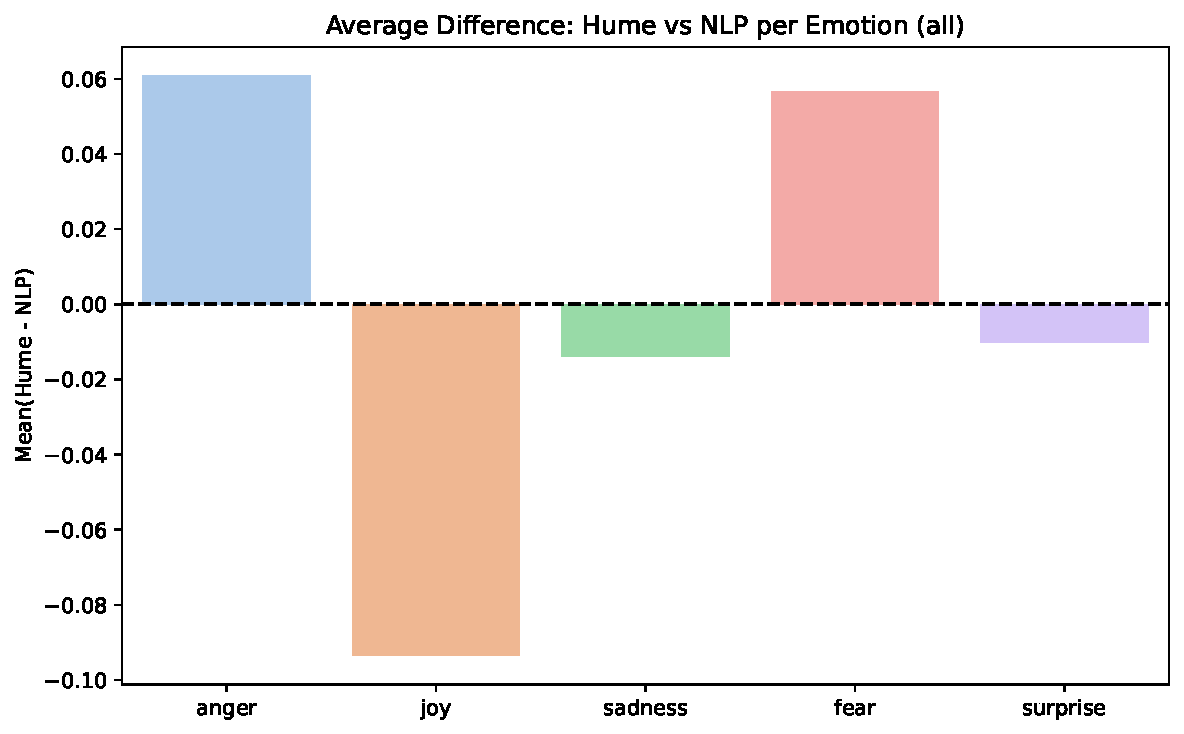
\includegraphics[width=0.7\textwidth]{png/results/rq2/hume_nlp_difference_all.pdf}
    \caption{Average difference in emotion scores between Hume AI and NLP Cloud}
    \label{fig:comp_bar_full_rq2}
\end{figure}

\newpage
\subsection{Statistical Analysis}
\subsubsection{Correlation Analysis}

To evaluate how text-based (NLP Cloud) and speech-based (Hume AI) emotion recognition aligns, Pearson correlation coefficients (r) were calculated for each emotion across all interview recordings. 
Table~\ref{tab:corr_all} presents the correlation values as well as corresponding p-values to examine the statistical significance. 

\begin{table}[H]
    \centering
    \caption{Pearson Correlations Between Vocal Feature and Hume AI Emotion Scores (All Recordings)}
    \label{tab:corr_all}
    \begin{tabular}{lrrl}
      \toprule
      \textbf{Emotion} & \textbf{Pearson r} & \textbf{p-value} & \textbf{Significant}\\
      \midrule
      Anger    & 0.466 & 0.007 & Yes \\
      Joy      & 0.521 & 0.002 & Yes \\
      Sadness  & 0.167 & 0.362 & No  \\
      Fear     & 0.171 & 0.348 & No  \\
      Surprise & 0.197 & 0.281 & No  \\
      \bottomrule
    \end{tabular}
  \end{table}


\begin{table}[H]
    \centering
    \caption{Pearson Correlations Between Vocal Feature and Hume AI Emotion Scores (Negative Recordings)}
    \label{tab:corr_neg}
    \begin{tabular}{lrrl}
      \toprule
      \textbf{Emotion} & \textbf{Pearson r} & \textbf{p-value} & \textbf{Significant}\\
      \midrule
      Anger    & 0.260 & 0.313 & No  \\
      Joy      & 0.556 & 0.020 & Yes \\
      Sadness  & 0.028 & 0.914 & No  \\
      Fear     & 0.270 & 0.294 & No  \\
      Surprise & 0.209 & 0.422 & No  \\
      \bottomrule
    \end{tabular}
  \end{table}
  

  \begin{table}[H]
    \centering
    \caption{Pearson Correlations Between Vocal Feature and Hume AI Emotion Scores (Positive Recordings)}
    \label{tab:corr_pos}
    \begin{tabular}{lrrl}
      \toprule
      \textbf{Emotion} & \textbf{Pearson r} & \textbf{p-value} & \textbf{Significant}\\
      \midrule
      Anger    & 0.160  & 0.568 & No  \\
      Joy      & 0.682  & 0.005 & Yes \\
      Sadness  & 0.546  & 0.035 & Yes \\
      Fear     & 0.098  & 0.729 & No  \\
      Surprise & -0.050 & 0.860 & No  \\
      \bottomrule
    \end{tabular}
  \end{table}

This data demonstrates a reasonable positive correlation for Anger(r = 0.468, p=0.0069) and Joy (r=0.521, p=0.0022), implying that these emotions are relatively consistent identified throughout the AI systems. 
The p-values (p<0.05) show a statistical significance and highlights a relevant relationship in how Anger and Joy are detected through different processes. 

Sadness, Fear, and Surprise show contrasted results with weak correlations (r<0.20) where the p-values indicate no significancy with low agreement between the AI models for these emotions. 
This suggest that text-based and speech-based emotion analysis have a higher disagreement when detecting these emotion expressions. 

Overall, some alignment for the more distinct emotions as Anger and Joy are declared through the correlation analysis, but some difficulties with consistent agreement are prominent for more nuances emotions as Sadness, Fear, and Surprise. 

\subsubsection{Paired t-Tests and Effect Sizes}
To further explore alignment and differences between speech-based (Hume AI) and text-based (NLP Cloud) emotion recognition, paired t-tests and Cohen's d were conducted. 
Table \ref{tab:t-test-all} shows the t-statistics, p-values, and Cohen's d for each emotion across the full dataset. Positive t-values implies that Hume rated that emotion more frequent than NLP, negative t-values suggest the opposite.
\begin{table}[!h]
    \centering
    \begin{tabular}{lllll}
    \multicolumn{5}{c}{\cellcolor[HTML]{C0C0C0}Full Dataset}                                                                                                                                                    \\
    \multicolumn{1}{c|}{\textbf{Emotion}} & \multicolumn{1}{c}{\textbf{t-statistic}} & \multicolumn{1}{c}{\textbf{p-value}} & \multicolumn{1}{c}{\textbf{Significant}} & \multicolumn{1}{c}{\textbf{Cohen's d}} \\ \hline
    \multicolumn{1}{l|}{Anger}            & 1,717                                    & 0,096                                & No                                       & 0,303                                  \\
    \multicolumn{1}{l|}{Joy}              & -1,726                                   & 0,0943                               & No                                       & -0,305                                 \\
    \multicolumn{1}{l|}{Sadness}          & -0,548                                   & 0,5876                               & No                                       & -0,097                                 \\
    \multicolumn{1}{l|}{Fear}             & 3,341                                    & 0,0022                               & Yes                                      & 0,591                                  \\
    \multicolumn{1}{l|}{Surprise}         & -0,657                                   & 0,5158                               & No                                       & -0,116                                
    \end{tabular}
    \caption{t-statistics, p-value with significance, and Cohen's d for all clips.}
    \label{tab:t-test-all}
\end{table}

Across all interviews, only Fear had statistically significant difference between the AI-models (t = 3.341, p = 0.0022), and had a medium effect size (Cohen's d = 0.591).
Hume AI rated fear consistently higher than NLP Cloud, which suggest a systematic difference in expression of vocal and textual for Fear. 

Even if differences were detected for Anger, Joy, Sadness, and Surprise, the variation was not statistically significant (p > 0.05), with small effect sizes (Cohen's d < 0.3). 
This indicates that regardless of minor divergences, the AI-models had relative alignment for recognizing these emotions, apart from Fear. 

\subsubsection{Conclusion Statistical Analysis}
Comparison of speech-based (Hume AI) and text-based(NLP Cloud) with statistical analysis demonstrates notable alignment, particularly for clear expressed emotions as Anger and Joy, 
which is confirmed by moderate to high degree of correlations. 
Emotions that are more subtle like Sadness, Fear, and Surprise, yet revealed low correlations, indicating modality-specifc distinctions. Paired t-tests strengthened this observation, pointing out Fear as the only emotion 
with statistically significant divergence where speech-based analysis assigned higher scores consistently. 
Overall, the analysis confirm that the AI modalities align in explicit emotional expressions but diverge when capturing nuanced emotional states. 
This highlight the strengths of the complementary use of speech- and text-based emotion recognition, each revealing unique features of emotional detection. 


\subsection{Sentiment-Based Analysis}
\label{sec:rq2-sentiment}
To explore how AI-based emotion recognition systems adapt to different emotional contexts, an sentiment-based analysis are conducted where the interviews are seperated by the design to provoke either positive or negative emotions.
The interviews followed an autobiographical recall approach, see \ref{sec:theo-interviews} Theoretical Framework, Interviews. 

While the interviews were structured to evoke either positive or negative emotions through different scenarios, it is important to note that these categorizations do not serve as a ground truth. 
Emotional expression, certainly in a conversational interview setting, may not fully align with the intended sentiment through the whole recording. 
Additionally, Hume AI analyzed vocal characteristics (how something is said), and NLP Cloud focuses on the semantic content of the transcription of the recording (what is said), which can have an impact on how each system interprets emotional tone. 

This analysis focuses on comparing Hume AI and NLP Cloud across positive and negative oriented interviews to investigate how each system 
acts to shifts in emotional context. 

\begin{figure}[!h]
    \centering
    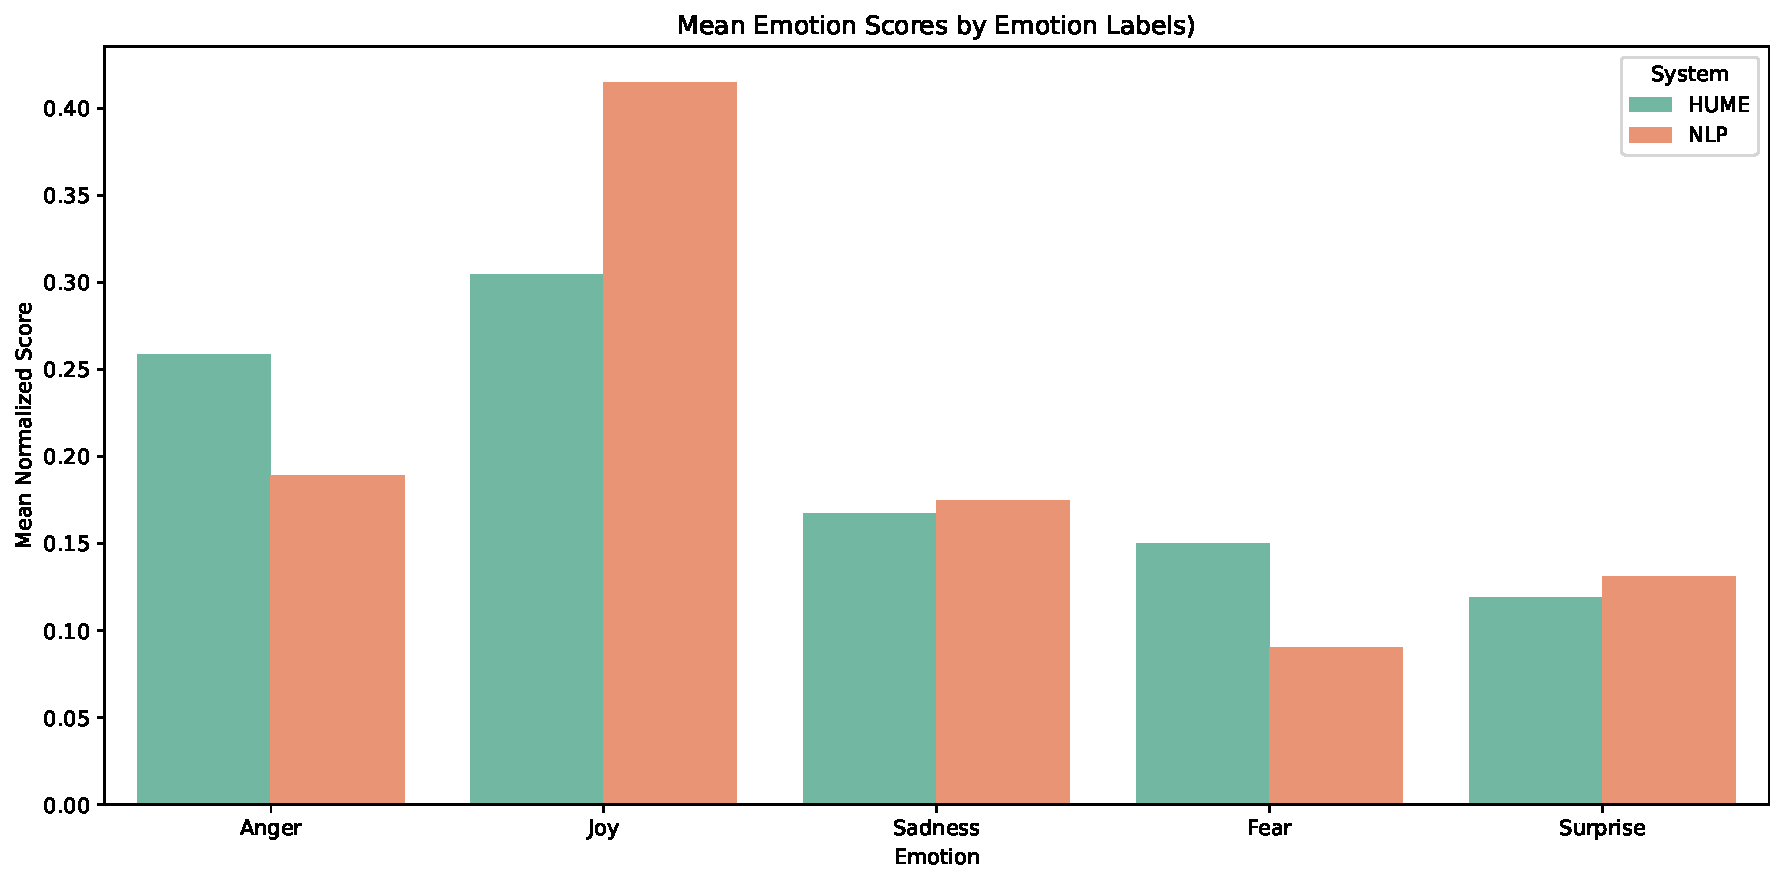
\includegraphics[width=0.7\textwidth]{png/results/rq2/sentiment_comparison_bar.pdf}
    \caption{Sentiment comparison bar for NLP and Hume.}
    \label{fig:sentiment-comp-rq2}
\end{figure}

\textbf{Positive Interviews Key Findings: }
Key Findings:
\begin{itemize}
    \item Anger was detected at significantly higher levels by Hume compared to NLP cloud, which rated Anger near zero. 
    This implies that Hume AI, that focuses on vocal tone, might pick up subtle vocal cues even when the participants are talking about positive memories. 
    NLP Cloud only analyzes textual content and does not interpret Anger when negative language is missing. 
    \item Joy is rated substantially high by NLP Cloud compared to both other emotions and Hume's probability. When participants discuss happy experiences, NLP 
    detects the emotion in high levels. Hume's lower detection for Joy might indicate that the expressed vocal features in the interview setting are less distinct,
    which leads to the underestimation. 
    \item Sadness and Fear are both rated higher than NLP, which gave these emotions minor scores. This aligns with that subtle negative undertones in speech, which could be due to reflective or 
    serious tones, are picked up by Hume in positive contexts. NLP misses these cues since nuances are not present in the transcribed content. 
    \item Surprise was detected at similar, low levels by both models. The emotion appears to be detected inconsistently, which may indicate that Surprise is difficult to capture, or rarely prominent in the recordings. 
\end{itemize}

\textbf{Negative Interviews Key Findings: }

\begin{itemize}
    \item Anger was somewhat higher rated by NLP than Hume. This indicate that NLP Cloud is sensitive to words expressed negatively, and may flag explicit language as anger. 
    Hume focuses on vocal tone, rated Anger slightly less, which can be due to vocal expressions being more controlled in an interview setting. 
    \item Joy was assigned higher by Hume than NLP in the negative interviews. Presumably due to the reason for the other emotions, where vocal patterns may be interpreted by Hume as positive even if its tied to a negative setting, 
    compared to NLP that devalued this emotion in comparison, probably because of negative transcriptions. 
    \item Sadness was detected at higher levels by NLP than Hume. 
    \item Fear and Surprise had similar detection results, with very small variation. This suggest that the emotions were expressed more consistently across both models, and the low levels that it might not be expressed prominent in the interviews overall. 
\end{itemize}

The text-based NLP Cloud is dependent on explicit emotional language, with highest rating for emotions that are clearly 
expressed in words, for example Joy in positive interviews, Anger and Sadness in negative interviews. 
The speech-based model Hume interprets vocal tones and may detect underlying emotional nuances, sometimes leading to unexpected results such 
as Joy in negative scenarios, Anger in positive scenarios. 

%%% T TESTS 
\subsubsection{Statistical Analysis}

Table \ref{tab:t-test-pos} demonstrates t-tests and Cohen's d for positive oriented interviews, where all emotions except for surprise shows significant differences 
with certainly large effect sizes. NLP have the aspects of overestimating Joy compared to Hume, where Hume in contrast tends to overestimate Anger in positive contexts. 
Hume rates Sadness and Fear more prominent than NLP, and Surprise remain inconsistent as previous results with no significant difference. 
The AI systems diverge significantly in positive interviews across almost all emotions, suggesting that text-based analysis can misinterpret 
emotional subtle cues, leading to inflating Joy. Hume may interpret vocal expressions in positive contexts as negative, probably due to the nature of the recordings, 
in agreement with previous results. 

 \begin{table}[!h]
    \centering
    \begin{tabular}{lllll}
    \multicolumn{5}{c}{\cellcolor[HTML]{C0C0C0}Positive Oriented Interviews}                                                                                                                                    \\
    \multicolumn{1}{c|}{\textbf{Emotion}} & \multicolumn{1}{c}{\textbf{t-statistic}} & \multicolumn{1}{c}{\textbf{p-value}} & \multicolumn{1}{c}{\textbf{Significant}} & \multicolumn{1}{c}{\textbf{Cohen's d}} \\ \hline
    \multicolumn{1}{l|}{Anger}            & 10,903                                   & 0                                    & Yes                                      & 2,815                                  \\
    \multicolumn{1}{l|}{Joy}              & -11,665                                  & 0                                    & Yes                                      & -3,012                                 \\
    \multicolumn{1}{l|}{Sadness}          & 6,177                                    & 0                                    & Yes                                      & 1,595                                  \\
    \multicolumn{1}{l|}{Fear}             & 5,125                                    & 0,0002                               & Yes                                      & 1,323                                  \\
    \multicolumn{1}{l|}{Surprise}         & -1,723                                   & 0,1069                               & No                                       & -0,445                                
    \end{tabular}
    \caption{t-statistics, p-value with significance, and Cohen's d for positive interviews.}
    \label{tab:t-test-pos}
\end{table}

Table \ref{tab:t-test-neg} presents conducted t-tests and Cohen's d in negative interviews, with significant differences for Joy, where Hume rates it significantly higher than NLP. 
In contrast, NLP has clear higher scoring for Sadness with large effects. 
Anger has a moderate difference, even if it is not statistically significant. No notable differences are detected for either Fear or Surprise. 
This implies that the AI systems strongly disagrees on Joy and Sadness detection in the negative contexts of the dataset. 

\begin{table}[!h]
    \centering
    \begin{tabular}{lllll}
    \multicolumn{5}{c}{\cellcolor[HTML]{C0C0C0}Negative Oriented Interviews}                                                                                                                                    \\
    \multicolumn{1}{c|}{\textbf{Emotion}} & \multicolumn{1}{c}{\textbf{t-statistic}} & \multicolumn{1}{c}{\textbf{p-value}} & \multicolumn{1}{c}{\textbf{Significant}} & \multicolumn{1}{c}{\textbf{Cohen's d}} \\ \hline
    \multicolumn{1}{l|}{Anger}            & -1,702                                   & 0,108                                & No                                       & -0,413                                 \\
    \multicolumn{1}{l|}{Joy}              & 3,72                                     & 0,0019                               & Yes                                      & 0,902                                  \\
    \multicolumn{1}{l|}{Sadness}          & -3,796                                   & 0,0016                               & Yes                                      & -0,921                                 \\
    \multicolumn{1}{l|}{Fear}             & 0,536                                    & 0,5993                               & No                                       & 0,13                                   \\
    \multicolumn{1}{l|}{Surprise}         & 1,311                                    & 0,2084                               & No                                       & 0,318                                 
    \end{tabular}
    \caption{t-statistics, p-value with significance, and Cohen's d for negative interviews}
    \label{tab:t-test-neg}
\end{table}

The emotional context impacts how the AI models detects emotions. Both systems presented larger differences in positive contexts, where vocal subtle cues and explicit language 
has different impact. 
NLP Cloud highly detects explicit emotions in text, especially Joy Anger and Sadness, but does not interpret subtle emotions such as Fear or Sadness in a positive context, since these emotions only might be expressed in nuanced vocal cues.
Hume AI captures these vocal nuances, resulting in detecting unexpected emotional states, such as Anger in positive interviews and Joy in negative ones. 
Which is affected by how something is said, where the tone can be opposing to the actual context. The speech-based model 
might overestimate negative emotions in reflective settings by this reason. 

Positive oriented interviews presents a wider divergence between the systems, which is confirmed by the large effect sizes. 
The negative interviews had more consistent detection, except for Joy and Sadness that had significant differences. 
For surprise, detection challenges or lack of expression of that emotion in the interviews might impacting the results of no significant difference for both sentiment contexts. 

\subsubsection{Conclusion Sentiment-Based Analysis}
In conclusion, the sentiment-based analysis shows that AI emotion detection in sensitive to both context and the modality. 
Text-based analysis has higher performance in identifying the explicit stated emotions, while speech-based 
analysis reveals deeper and probably more subtle emotional cues. 
These results suggests that none of the systems provides a universally accurate interpretation across all emotions,
which indicates that text and speech-based emotion detection has limitations. 


\subsubsection{Case Example}
single clip comparison 

breifly illustrate how speech vs text differ in practice 

\subsection{Conclusion of RQ2 Data Analysis}
The results of this research question show that even if Hume AI and NLP Cloud partially aligns in detecting emotions, certainly for clearly expressed emotions such as Anger and Joy, 
they diverge significantly in their predictions of more nuanced emotions such as Fear, Sadness, and Surprise. Statistical tests confirmed a significant difference for Fear. 
Sentiment-based analysis showed that emotional context have an impact on the results, when analysing five basic emotions, where positive scenarios had a larger model divergence. 
As discussed above, the interview setting and overall data collection may have different impacts on the results. Still, the findings highlights how speech- and text-based models are complementary, each 
with their own strenghts to capture different aspects of emotion expression, and indicate that relying on a single modality could have limitations for comprehensive emotion detection in speech.  


%%%%%%%%%%%%%%%%%%%%%%%%%%%%%%%%%%%%%%%%%%%%%%%%%%%%%%%%%%%%%%%%%%%%%%%%%%%%%%%%%%%%%%%%%%
                        %%%%%%%%%%%%%%%%%%%%% RQ3   %%%%%%%%%%%%%%%
%%%%%%%%%%%%%%%%%%%%%%%%%%%%%%%%%%%%%%%%%%%%%%%%%%%%%%%%%%%%%%%%%%%%%%%%%%%%%%%%%%%%%%%%%%
\section{Data Analysis for RQ3: AI and self-assessed emotion labels}

The third research question explores how AI-generated emotion labels - from both speech-based (Hume AI) and text-based (NLP Cloud) 
analyses - aligns with self-assessed emotions. It is of importance to understand how these AI systems reflect humans perception of 
their own emotions and explore how the systems align with the participants own emotional viewpoint.  
To answer this question, participants own assessments are compared with AI-labels to gain an understanding if these systems are aligned with human self-perception of their emotions and how the modality affects the results. 
To explore alignment and divergence, the analysis include comparisons of average scoring, correlations, statistical analysis, and sentiment separation.  
\subsection{Descriptive Overview}

For an initial overview, Table~\ref{tab:summery-rq3} summerizes the average emotion scores across all 32 interview recordings 
for each emotion category (Anger, Joy, Sadness, Fear, Surprise). The table presents mean values and standard deviation for self-resported scores 
aside both AI-systems.

\begin{table}[!h]
    \centering
    \begin{tabular}{c|llllll}
    \textbf{Emotion}  & \multicolumn{1}{c}{\textbf{Self Mean}} & \multicolumn{1}{c}{\textbf{Hume Mean}} & \multicolumn{1}{c}{\textbf{NLP Mean}} & \multicolumn{1}{c}{\textbf{Self Std}} & \multicolumn{1}{c}{\textbf{Hume Std}} & \multicolumn{1}{c}{\textbf{NLP Std}} \\ \hline
    \textbf{Anger}    & 0,21                                   & 0,26                                   & 0,2                                   & 0,124                                 & 0,072                                 & 0,223                                \\
    \textbf{Joy}      & 0,312                                  & 0,302                                  & 0,396                                 & 0,2                                   & 0,117                                 & 0,351                                \\
    \textbf{Sadness}  & 0,19                                   & 0,167                                  & 0,181                                 & 0,105                                 & 0,065                                 & 0,138                                \\
    \textbf{Fear}     & 0,136                                  & 0,15                                   & 0,093                                 & 0,061                                 & 0,045                                 & 0,092                                \\
    \textbf{Surprise} & 0,149                                  & 0,118                                  & 0,129                                 & 0,082                                 & 0,022                                 & 0,089                               
    \end{tabular}
    \caption{Mean and standard deviation for Hume, NLP, and Self-labels for the full dataset.}
    \label{tab:summery-rq3}
\end{table}

As shown in the table, Joy consistently has the highest average scores across all sources, in certain for NLP Cloud,
which has a notable higher mean value (0.396) compared to self-reports (0.312) and Hume (0.302). 
In contrast, emotions as Fear and Surprise have a tendency for lower average scores, where both AI-systems generally assigns these 
emotion labels slightly lower for these emotions compared to the participants own scoring. 

To visualize these differences, Figure~\ref{fig:comp-bar-rq3-all} illustates a bar chart that compares the average emotion scores defined by 
participants self-assessment, Hume AI and NLP Cloud. 

\begin{figure}[!h]
    \centering
    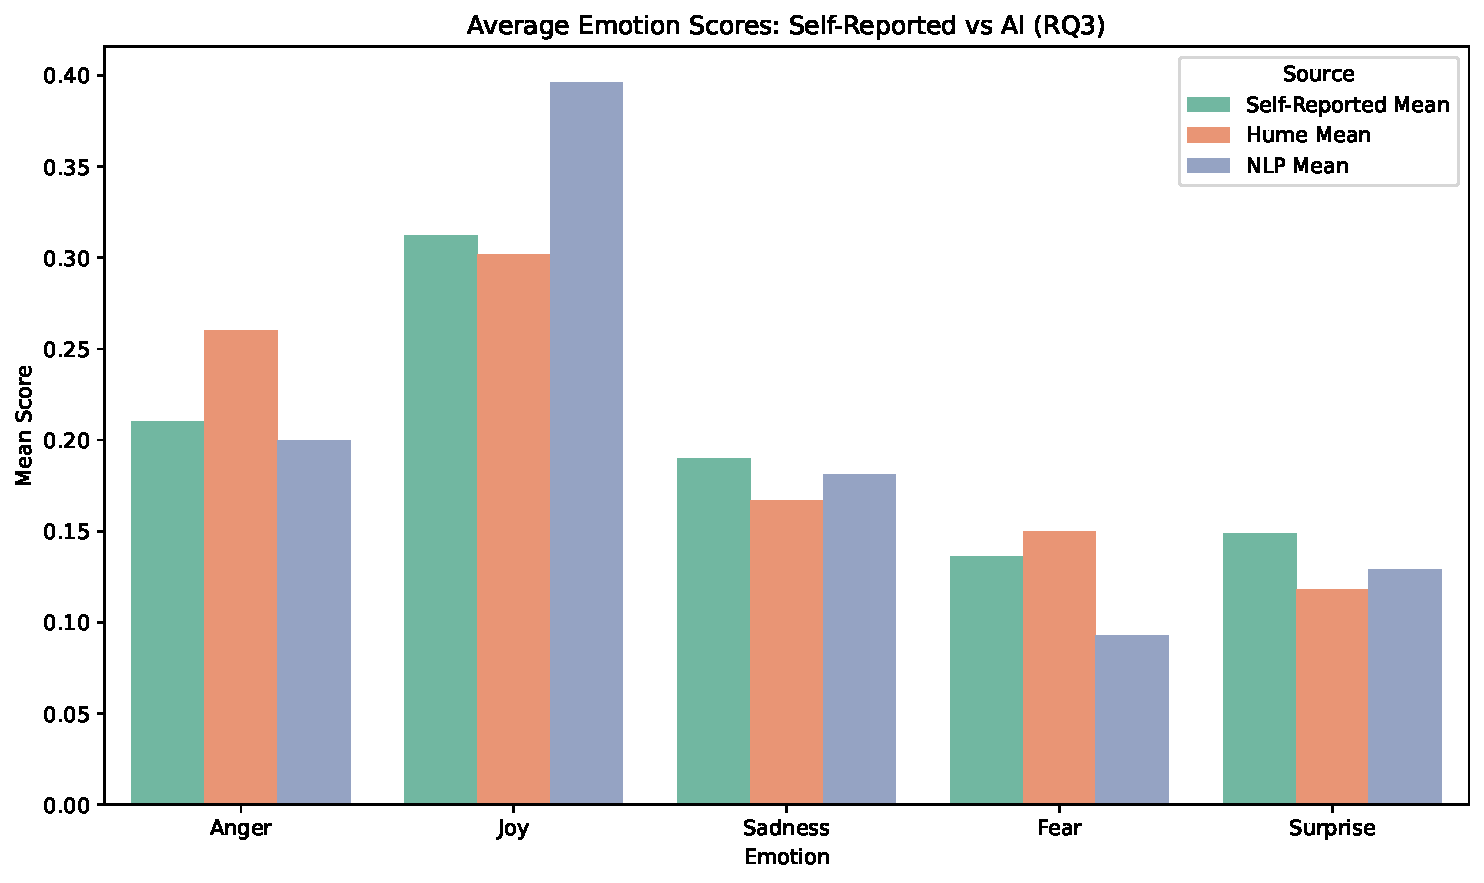
\includegraphics[width=0.7\textwidth]{png/results/rq3/rq3_emotion_comparison.pdf}¨
    \caption{Comparison of emotional labels for Hume, NLP, and self-assessed.}
    \label{fig:comp-bar-rq3-all}
\end{figure}

Key patterns from bar chart \ref{fig:comp-bar-rq3-all}:
\begin{itemize}
    \item NLP Cloud tends to overestimate Joy compared to both self-reported and Hume's emotion labeling. 
    \item For Anger, self and NLP-labeling are highly congurent, while Hume assigns higher average scores.
    \item Regarding Sadness and Surprise, the AI systems tends to report moderately lower scores than the participants, particularly for Surprise. 
    \item Sadness, Fear, and Surprise are consistently rated lower across all sources, especially Fear and Surprise, where Hume tends to rate Fear more frequent than the other, and self-labels has a higher surprise score than the other sources.
\end{itemize}
This comparison suggests that even if general alignment in emotional ranking occur, where Joy is most prominent across all sources, both AI systems 
demonstrate differences compared to human self-perception. Particularly NLP Cloud that appears to be more prone to rating Joy, while Hume provides more moderate scores, although all sources tends gravitate towards high scores for emotions Anger and Joy. 

These insights compose the framework for further statistical analysis, where correlation analysis and significance tests will 
be used to evaluate the strenghts and consistency of these patterns. 

\subsection{Correlation and Visual Analysis}
To evaluate the alignment between AI-generated emotion scores and participants self-reported emotions, 
Pearson correlation analyses were conducted across the five emotion categories for both speech-based (Hume AI) and text-based (NLP Cloud) compared to self-reporting.
With these measurements the relationship's strength and direction and the statistical significance can be reviewed. 

\subsubsection{Hume AI vs Self-Reported Emotions}
The correlation results for Hume AI is demonstrated in Table~\ref{tab:corr-hume-self}, and indicate generally weak correlations across the majority of emotions. 
Anger is the only emotion showing a statistic significant correlation (r = 0.359, p = 0.043), which indicates a moderate alignment between Hume AI's speech based emotion 
detection and participants own perception for this emotion. Other emotions, such as Fear (r = 0.007, p = 0.969), presents no relevant correlation. 

It is of importance to note that Hume AI analyzes vocal expression patterns, such as vocal bursts and porosody, rather than the semantic content of the recorded speech. 
Considering the interview setting that the recordings which complies the data collection, where participants recalled past emotional experiences in a controlled environment, 
the extent to which emotions were expressed vocally may vary, that potentially incluence the correlation results. 

%%% Correlation hume self 

\begin{table}[!h]
    \centering
    \begin{tabular}{cll}
    \multicolumn{3}{c}{\cellcolor[HTML]{C0C0C0}Hume vs Self-Assessed}                                                        \\
    \multicolumn{1}{c|}{\textbf{emotion}}  & \multicolumn{1}{c}{\textbf{pearson\_r}} & \multicolumn{1}{c}{\textbf{p\_value}} \\ \hline
    \multicolumn{1}{c|}{\textbf{anger}}    & 0,359                                   & 0,043                                 \\
    \multicolumn{1}{c|}{\textbf{joy}}      & 0,334                                   & 0,062                                 \\
    \multicolumn{1}{c|}{\textbf{sadness}}  & 0,050                                   & 0,784                                 \\
    \multicolumn{1}{c|}{\textbf{fear}}     & -0,007                                  & 0,969                                 \\
    \multicolumn{1}{c|}{\textbf{surprise}} & 0,088                                   & 0,631                                
    \end{tabular}
    \caption{Correlation and p-value for Hume AI and self reporting.}
    \label{tab:corr-hume-self}
\end{table}

%%% Self vs NLP 
\subsubsection{NLP Cloud vs Self-Reported Emotions}
\label{sec:nlp-self}
NLP Cloud demonstrated strong and statistically significant correlations for four of five emotions, see 
Table~\ref{tab:corr-nlp-self}. 

\begin{table}[!h]
    \centering
    \begin{tabular}{cll}
    \multicolumn{3}{c}{\cellcolor[HTML]{C0C0C0}NLP vs Self-Assessed}                                                         \\
    \multicolumn{1}{c|}{\textbf{emotion}}  & \multicolumn{1}{c}{\textbf{pearson\_r}} & \multicolumn{1}{c}{\textbf{p\_value}} \\ \hline
    \multicolumn{1}{c|}{\textbf{anger}}    & 0,739                                   & 0,00000                               \\
    \multicolumn{1}{c|}{\textbf{joy}}      & 0,863                                   & 0,00000                               \\
    \multicolumn{1}{c|}{\textbf{sadness}}  & 0,710                                   & 0,00001                               \\
    \multicolumn{1}{c|}{\textbf{fear}}     & 0,669                                   & 0,00003                               \\
    \multicolumn{1}{c|}{\textbf{surprise}} & 0,092                                   & 0,61569                              
    \end{tabular}
    \caption{Correlation and p-value for NLP Cloud and self reporting.}
    \label{tab:corr-nlp-self}
\end{table}

Key Findings: 
\begin{itemize}
    \item Joy showed a very strong correlation (r = 0.863, p < 0.0001). 
    \item Anger and Sadness had very high correlation values (Anger: r = 0.793, Sadness: 0.710), with extremely low p-values for both emotions. 
    \item Fear had a moderately strong correlation (r = 0.67, p = 0.00003), with considerably statistical significance. 
    \item Surprise had no statistical significance and weak correlation (r = 0.092, p = 0.616). 
\end{itemize}
Text-based emotion detection with NLP shows a explicit correlation with self-reported emotions for four out of five emotions. The emotion scoring certainly similar for Anger, Joy, Sadness and Fear. 
Surprise was the only emotion that did not show a significant correlation for NLP and self-perceived emotion labels. Surprise is the one emotion both AI-systems concurrently failed to show a significant correlation, 
which suggests that the models have difficulties in detect these emotions accurately. However, this inconsistency may not reflect limitations of the 
AI-systems. During data collection, several participants expressed challenges in assessing their level of Surprise and had difficulties understanding how to rate that emotion, 
this indicates both potential variablity and misunderstanding in self-reported scores for Surprise. 
Therefore, the low correlation for Surprise could be associated to unreliable self-assessments, rather than a underlying weakness in AI-based detection. 


\subsubsection{Visual Correlation}
Figure \ref{fig:scatter-anger-rq3} illustrates the correlation between self-reported Anger scores and AI-labeled predictions. As shown, Hume AI shows a weak to moderate positive tendency (r = 0.36, p = 0.043), still reaches statistical significance, even if the data points are more dispersed around the trend line. 
In contrast, NLP Cloud shows a strong and statistical significant correlation (r = 0.74, p < 0.0001), which is visually very noticable with the tightly clustered linear relationship. 

%% ANGER
\begin{figure}[!h]
    \centering
    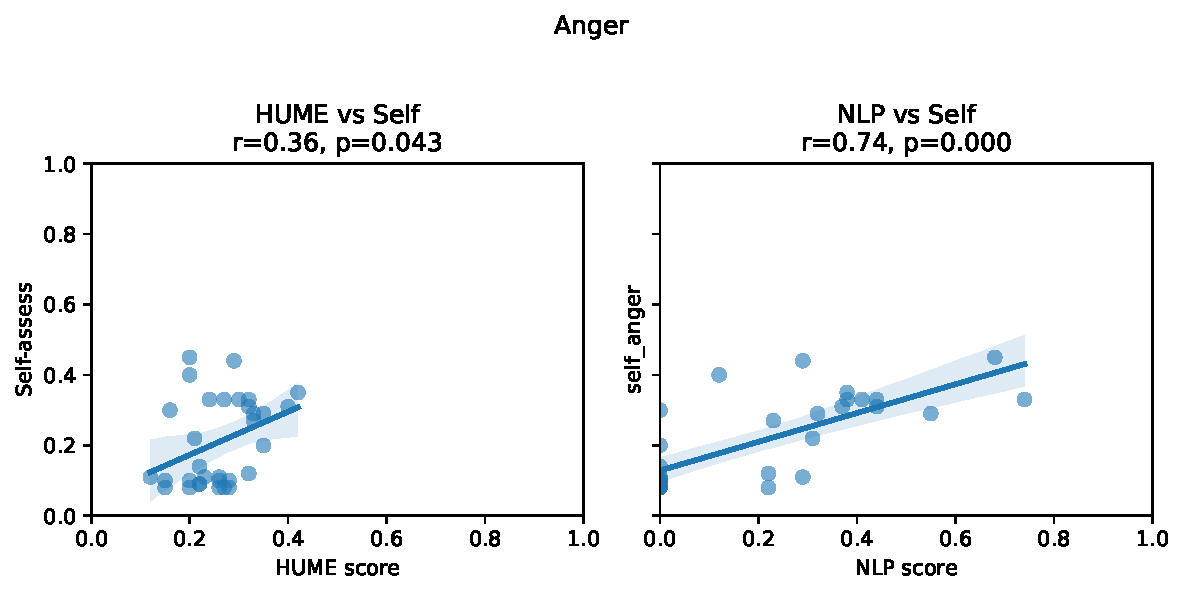
\includegraphics[width=0.7\textwidth]{png/results/rq3/scatter_anger_vs_self.pdf}
    \caption{Scatter plot, Hume, NLP vs. Self for Anger.}
    \label{fig:scatter-anger-rq3}
\end{figure}

Figure \ref{fig:scatter-joy-rq3} demonstrates the Joy correlation between self-reports and AI-predictions. Similar to Anger, Hume AI presents a weak to moderate positive trend (r = 0.33, p = 0.062), however it does not reach statistical significance. The diagram illustrates a disperse for the data points comparable to Anger.
As stated in previous results, NLP Cloud reveal a prominent statistical correlation (r = 0.86, p < 0001), clearly presented in the diagram. 
%% JOY
\begin{figure}[!h]
    \centering
    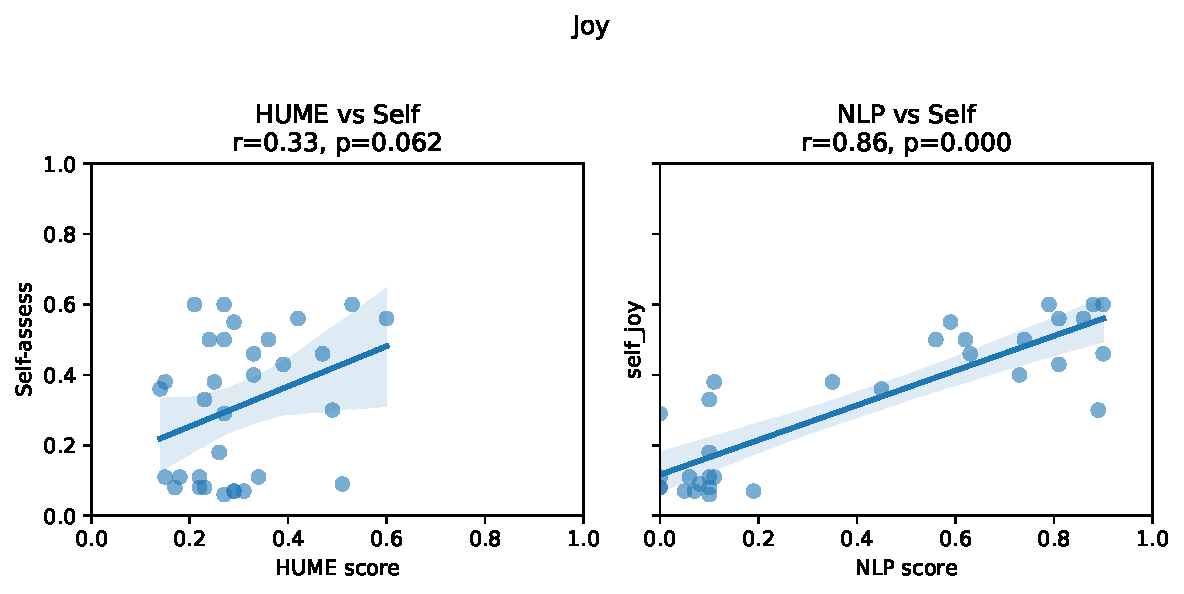
\includegraphics[width=0.7\textwidth]{png/results/rq3/scatter_joy_vs_self.pdf}
    \caption{Scatter plot, Hume, NLP vs. Self for Joy.}
    \label{fig:scatter-joy-rq3}
\end{figure}
\medskip

Figure \ref{fig:scatter-surprise-rq3} presents the correlation results for Surprise. Both Hume AI and NLP Cloud has minor correlation with self-reported Surprise scoring (r = 0.09), the lack of alignment is reflected in the scattered plots where no direct clear linear trend is shown. 
As stated in \ref{sec:rq2-sentiment} RQ2, Sentiment-Based Analysis, the inconsistent results may be due to Surprise being slighter expressed during the interviews. For this research question, it is important to note that several participants expressed confusion about how to interpret and answer 
their experienced Surprise, which can affect these inconsistent outcomes. 
%% SURPRISE 
\begin{figure}[!h]
    \centering
    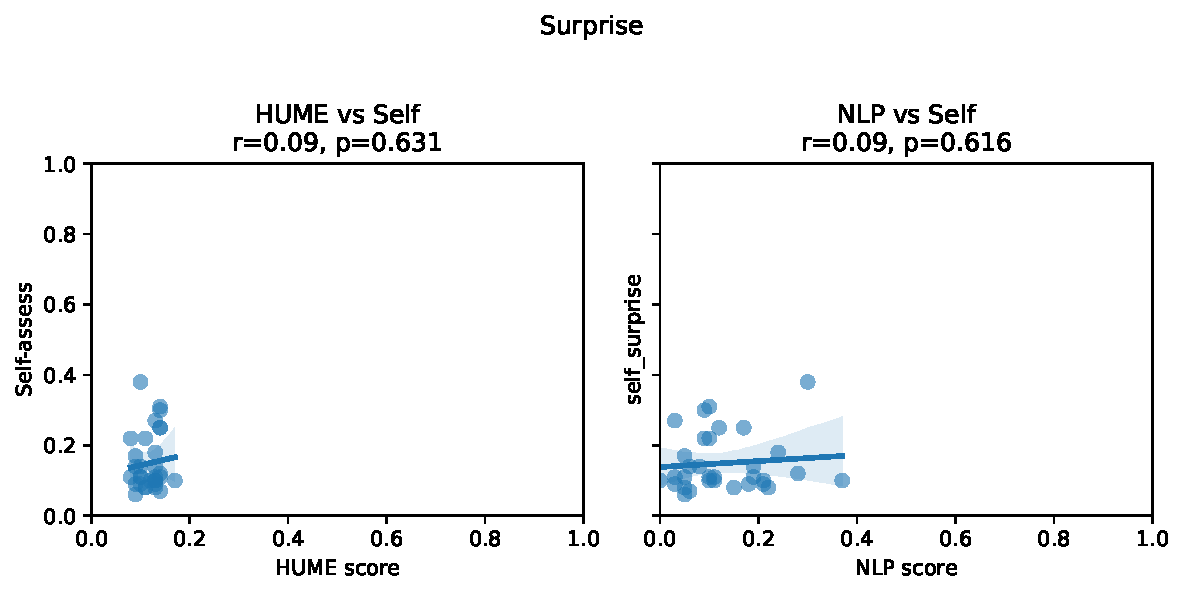
\includegraphics[width=0.7\textwidth]{png/results/rq3/scatter_surprise_vs_self.pdf}
    \caption{Scatter plot, Hume, NLP vs. Self for Surprise.}
    \label{fig:scatter-surprise-rq3}
\end{figure}

The scatter plots support previous presented statistical findings, highlighting the higher consistency of alignment between NLP Cloud and participant assessment for explicit expressed emotions as Joy and Anger. 
The shared difficulty of both models in detecting Surprise is presented further, possibly due to participant misunderstanding or that the interview scenarios were not oriented directly towards Surprise. 

\subsubsection{Conclusion Correlation and Visual Analysis}
This section reveal a clear trend, both statistically and visually: NLP Cloud aligns strongly with self-reported emotions for four out of five emotions, Anger, Joy, Sadness, and Fear, while Hume has weaker and 
non-significant correlations except for Anger. Both AI-models show weak levels of detecting Surprise, likely due to the interview setting and participant understanding of the question. 
These results emphasize the strength of text-based emotion analysis for recognition of explicit verbally emotional states, often aligned with self-reports, and 
implies that vocal-based interpretation within reflective interview setting may have difficulties, particularly in comparison to the participants own perceived emotion states. 

\subsection{Statistical Analysis and Effect Sizes}

To explore if AI-generated emotion scores has a significant difference from self-reported emotions, paired t-tests were conducted for both Hume AI and NLP Cloud across each emotion. 
To evaluate the effect size of these differences, Cohen's d were calculated. These results are presented in Table~\ref{tab:t-test-rq3}.
\begin{table}[!h]
    \centering
    \begin{tabular}{l|lllll}
    \textbf{System} & \textbf{Emotion} & \textbf{t-statistic} & \textbf{p-value} & \textbf{Significant} & \textbf{Cohen's d} \\ \hline
    HUME            & Anger            & 2,399                & 0,023            & Yes                  & 0,424              \\
    NLP             & Anger            & -0,373               & 0,711            & No                   & -0,066             \\
    HUME            & Joy              & -0,271               & 0,788            & No                   & -0,048             \\
    NLP             & Joy              & 2,331                & 0,026            & Yes                  & 0,412              \\
    HUME            & Sadness          & -1,069               & 0,293            & No                   & -0,189             \\
    NLP             & Sadness          & -0,525               & 0,603            & No                   & -0,093             \\
    HUME            & Fear             & 1,052                & 0,301            & No                   & 0,186              \\
    NLP             & Fear             & -3,496               & 0,001            & Yes                  & -0,618             \\
    HUME            & Surprise         & -2,109               & 0,043            & Yes                  & -0,373             \\
    NLP             & Surprise         & -1,011               & 0,320            & No                   & -0,179            
    \end{tabular}
    \caption{T-statistics, p-value and Cohen's d for AI-models and self-assessed emotions.}
    \label{tab:t-test-rq3}
\end{table}

\textbf{Key Findings:}
\begin{itemize}
    \item Hume AI: 
    \begin{itemize}
        \item Anger (p = 0.023) and Surprise (p = 0.043) showed significant differences. 
        \item Both Anger and Surprise showed small to moderate effect sizes (Cohen's d > 0.4), which suggests that Hume AI tends to overestimate Anger and underestimate Surprise compared to self-reported emotion scores. However, as declared in NLP vs. Self-Reported emotions~\ref{sec:nlp-self}, particpants stated confusion regarding assessing Surprise.
        \item For the other emotions, Joy, Sadness, and Fear, no significant differences were found, suggesting closer average alignment for these emotions.
    \end{itemize}
    \item NLP Cloud: 
    \begin{itemize}
        \item Joy (p = 0.026) and Fear (p = 0.001) presented significant differences. 
        \item Fear had a particularly evident difference, (Cohen's d = -0.618) states a medium-to-large effect size, indicating that NLP Cloud underestimated Fear compared to self-reported emotion scores. 
        \item Joy had a small-to-moderate effect size (Cohen's d = 0.412), suggesting that NLP overestimated Joy compared to the participants own perception. 
        \item Anger, Sadness, and Surprise showed no significant difference. 
    \end{itemize}
\end{itemize}
\textbf{General Analysis:}

Both AI systems demonstrates some alignment with self-reported emotions, the results indicate certain biases. Self reported emotion scores appears to be more prone to diverge from Hume AI's detection of Anger and Surprise. 
Regarding NLP Cloud, the emotion scores are distinct from self-assessed emotions for Fear and Joy, where Fear is most prominent. This could indicate either challenges in text-based detection of these subtle, negative emotions, 
or challenges for the participants to assess these emotions. 

Even where statistical significance is found, the effect size implies that most differences are small to moderate, which 
suggests that even if deviations exists, they are not disturbingly large. It is no consistent significant difference for the AI-systems across all emotions, proposing that AI performance may vary depending on emotional category and the method (speech vs text, and different AI-models).
However, it is important to emphasize that these results may not fully reflect the performance or accuracy of the
AI models, as the analysis are based on a small dataset with semi-structured interviews. Furthermore, disparity and miscalculations may arise from challenges participants experienced in assessing their own emotions after each interview. 

\medskip
Overall, these findings suggest that AI systems can approximate human emotional self-assessment with partial alignment, some differences still appear depending on emotion and detection method. 
Hume AI had more diverse scores for Anger and Surprise, while NLP Cloud was more distinct for Fear and Joy. The differences may reflect some challenges in AI detection or difficulties for the participants to assess their emotions accurately. 

Even if some differences were significant statistically, the effect sizes indicate that they are generally small to moderate. There is no consistent pattern across all emotions which indicates that the AI performance vary by emotion category and analysis method (speech vs text).
\medskip

Considering the small dataset, the subjective nature of self-assessment, and the recording circumstances of the interview setting, these findings should be interpreted 
carefully and should be seen as exploratory and not conclusive. 


%%%%% SENTIMENT rRQ3 %%%%%% 
\subsection{Sentiment-Based Analysis}
To explore how AI-generated emotion labels and self-reported emotions align, a sentiment-based analysis have been conducted through seperation of negative and positive interviews. 
Each participant reported scores (1-6 scale, normalized to 0-1) for all five emotions after each interview-scenario, to provide a subjective component to compare with AI predictions.   

Figure~\ref{fig:sentiment-bar-rq3} illustrate the average emotion scores for positive and negative interviews for Hume AI, NLP Cloud, and self-assessment. 
When interpreting these results, it is important to note that participants actual emotional expressions, particularly vocally, may not be fully aligned with the intention to evoke distinct emotional tones, due to the reflective and conversational nature of the setting.
\begin{figure}[!h]
    \centering 
    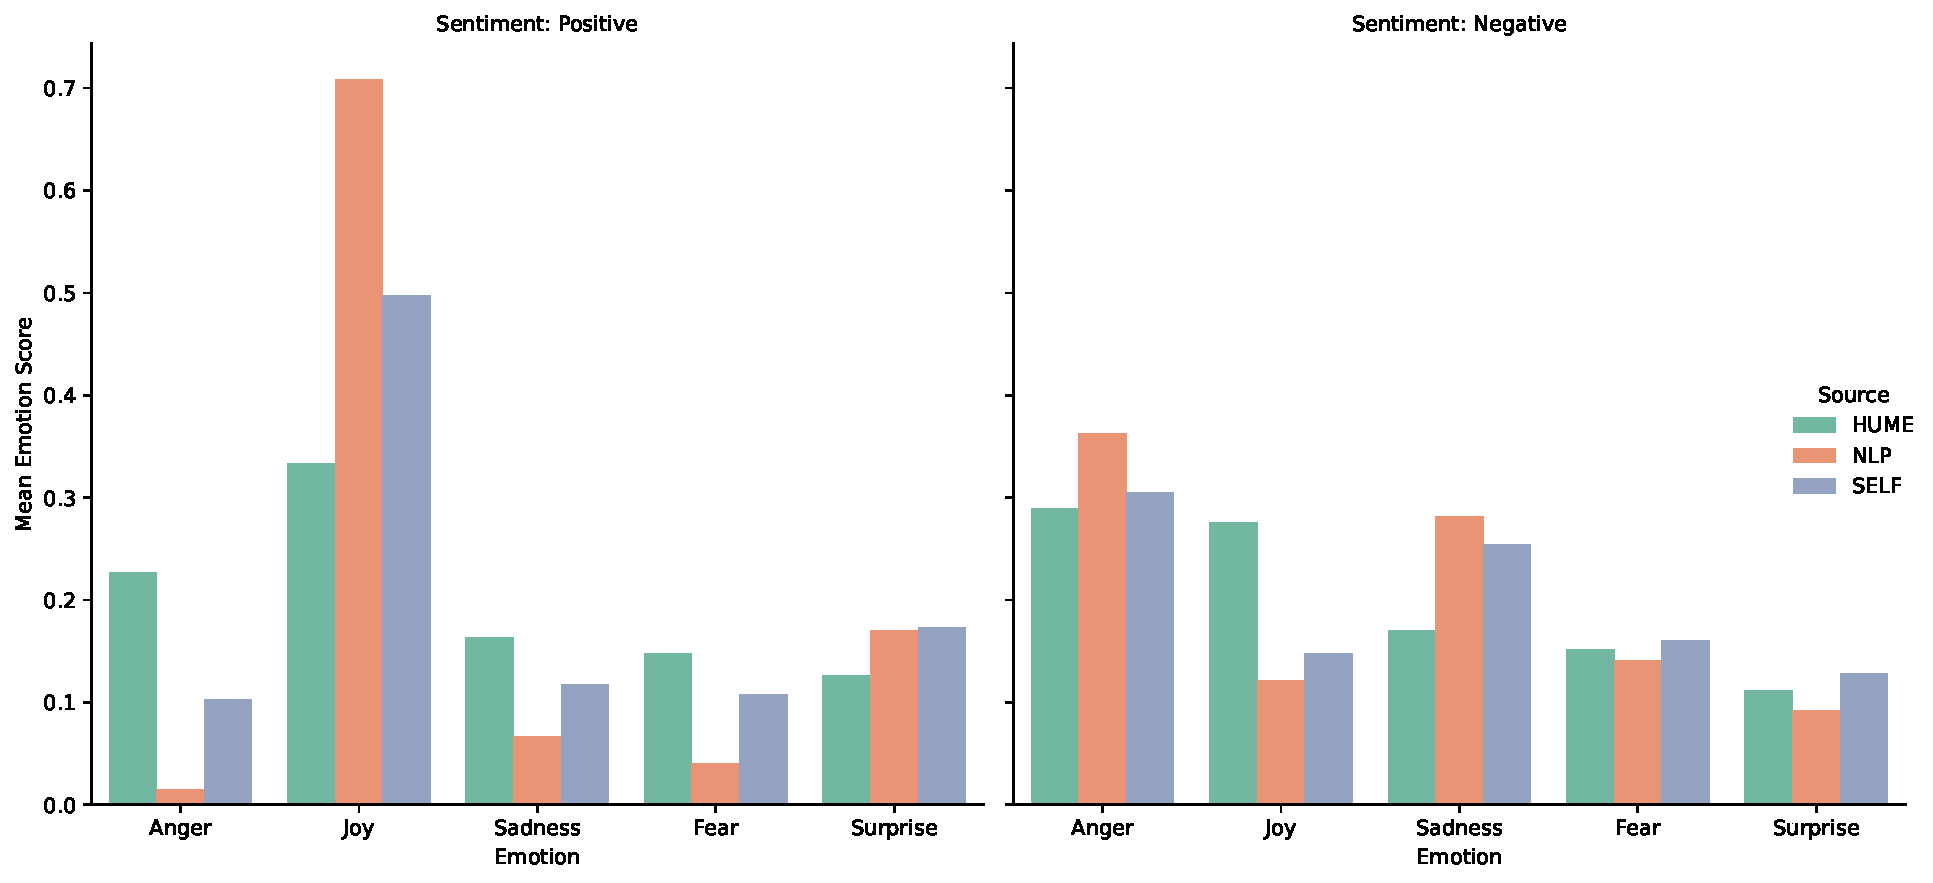
\includegraphics[width=0.7\textwidth]{png/results/rq3/rq3_sentiment_grouped_bar.pdf}
    \caption{Emotion scores for all sources grouped by sentiment.}
    \label{fig:sentiment-bar-rq3}
\end{figure}

\textbf{Positive Interviews}
\begin{itemize}
    \item Joy was highly self-reported consistently, which aligns closely with NLP Cloud's text-based ratings, but considerably higher than Hume AI's vocal analysis. 
    This alignment suggest that participants expressed positive emotions verbally, which was captured by NLP Cloud effectively. The lower Hume ratings for Joy indicate a divergence since vocal expressions of Joy in 
    the reflective, interview setting may be less pronounced and therefore harder for the speech-based model to detect. 
    \item The negative emotions (Anger, Sadness, Fear) were assessed at lower levels by participants, as expected for positive oriented interviews. Self-assessments generally matched Hume's higher detection of subtle negative emotion expressions better than NLP's minor ratings. 
    This aligns with the idea that participants may express suble negative tones unintentionally in their voice, even if the participants perceived their emotions as predonimantly positive. 
    \item Surprise showed moderate self-report levels, more close agreed to NLP and slighly less alignment with Hume, reflecting inconsistency in vocal vs. textual emotion cues.  
\end{itemize}
In positive interviews, NLP Cloud consistently rated Joy higher, in agreement with previous results. The difference from self-reported joy is similar, although NLP tends to rate it moderately higher. 
This reflect the strength of text-based detection for explicit positive sentiment when analyzed as a transcription. 

\medskip
\textbf{Negative Interviews}
\begin{itemize}
    \item Anger and Sadness were reported at higher levels by participants, which reflects the intention of the interview of recalling negative emotions. Both AI models were aligned with self-reports for Anger, even if NLP rated it somewhat higher, 
    probably due to explicit negative language in transcriptions. Sadness showed stronger alignment with NLP than Hume, indicating explicit expressed sadness-related emotions verbally. 
    \item Joy was reported low by participants, but frequently assigned higher by Hume than the other sources. Suggesting that vocal features were interpreted as positive by Hume might not align with subjective emotional experiences, 
    showing a clear divergence between vocal emotion cures and participants own perception. 
    \item Fear and Surprise showed low levels consistently across self-reports and both AI-models, indicating that these emotions were less expressed or experiences, resulting in minimal discrepancies. 
\end{itemize}

These results emphasize that emotional expression is complex in conversational settings, showing that textual anlyses track explicit articulated emotions, 
while speech-based analyses reveal less intentionally expressed emotional nuances, sometimes in disagreement with participants subjective assessments. 

The sentiment-based comparison clearly presents that emotional expression and self-awareness have a signficant variance between modalities. Explicit emotions articulated in words are closely aligned between self-assessed rating and text-based analysis. 
while implicit or suble emotions expressed through vocal tone have a notable divergence. This highlights that AI modalities complement rather than duplicate emotional understanding. 
Speech-based models provide insights into emotional subtleties that might be unconscious to the participant, while text-based analyses capture verbalized emotions closely to subjective experiences. 


\subsection{Conclusion of RQ3 Data Analysis}
The results show that both systems have partial alignment with self-reported emotions, however, the correlation varies depending on emotion and modality. 
Text-based (NLP Cloud) presented a strong alignment with participants own perception for clear verbally expressed emotions like Joy And Anger. Subtler vocal cues were interpreted by the speech-based 
model (Hume AI), which may not always reflect self-perceived emotions. Emotions like Fear and Surprise had most visiable differences for both AI models. 
Overall, the results implies that speech- and text-based emotion recognition comprehend different layers of expressed emotions, suggesting that complementary use of modalities can offer a more nuanced understanding.  